\section{Streams}\label{sec:streams}

\subsection{Streams and stream operators}\label{sec:notation}

$\N$ is the set of natural numbers, $\B$ is the set of Booleans, and $\Z$ is the set of integers.
$[n] = \{ 0, 1, 2, \ldots n-1 \}$ is the set of natural numbers less than n.

\begin{definition}[stream]
Given a set $A$, a \defined{stream} \emph{of values from $A$}, or an \emph{$A$-stream}, is a function $\N \rightarrow A$. 
We denote by $\stream{A} \defn \{ s \,|\, s : \N \to A \}$ the set of all $A$-streams. 
\end{definition}

When $s\in\stream{A}$ and $t\in\N$ we 
write $s[t]$ for the $t$-th element of the stream $s$ instead of the usual $s(t)$
to distinguish it from other function applications.

We usually think of the index $t\in\N$ as (discrete) time and of $s[t]\in A$ 
as the value of the the stream $s$ ``at time'' $t$.

For example, the stream of natural numbers given by $\id[t] = t$ is the sequence of values
$\sv{0 1 2 3 4}$.

\begin{comment}
\begin{definition}
A \defined{finite stream} with $n$ values from $A$ is a function $[n] \to A$.
\end{definition}

A prefix of a stream is a finite stream.  For example, the prefix of $\id$ containing 
the first 5 values is the finite stream 
$[\begin{array}{ccccc} 0 & 1 & 2 & 3 & 4 \end{array}]$.
\end{comment}

\begin{definition}[stream operator]
A (typed) \defined{stream operator} with $n$ inputs is a function $T:\stream{A_0}\times\cdots\times\stream{A_{n-1}}\to\stream{B}$. 
\end{definition}

In general we will use ``operator'' for functions on streams, and
``function'' for computations on ``scalar'' values.

We are using an extension of the simply-typed lambda calculus to write \dbsp programs;
we will introduce its elements gradually.  However, we find it more readable to
also use signal-processing-like circuit diagrams to depict \dbsp programs,
as in Figure~\ref{fig:stream}.

Stream operator \emph{composition} (function composition) is shown as chained circuits.
The composition of a binary operator $T: \stream{A} \times \stream{B} \to \stream{A}$ with the 
unary operator $S: \stream{A} \to \stream{B}$ into the computation 
$\lambda s. T(T(s,S(s)),S(s)) : \stream{A}\to\stream{A}$ 
is given by the following circuit:

\begin{center}
\begin{tikzpicture}[auto,>=latex,minimum width=.5cm]
  \node[] (input) {$s$};
  \node[] [right of=input] (dummy) {};
  \node[block, below of=dummy] (S1) {$S$};
  \node[block, right of=S1] (T1) {$T$};
  \node[block, right of=T1] (T2) {$T$};
  \node[block, above of=T2] (S2) {$S$};
  \node[right of=T2] (output) {$o$}; 
  \draw[->] (input) -| (S1);
  \draw[->] (input) -| (T1);
  \draw[->] (S1) -- (T1);
  \draw[->] (T1) -- (T2);
  \draw[->] (input) |- (S2);
  \draw[->] (T2) -- (output);
  \draw[->] (S2) -- (T2);
\end{tikzpicture}
\end{center}

Arrows with a single start and multiple 
ends denote a stream that is reused multiple times, e.g., $s$
in the above diagram is used 3 times.  Diagrams, however, do obscure the
ordering of the inputs of an operator; in the above examples
we have to indicate which ones are the first and respectively second inputs of $T$
if $T$ is not commutative.  Most of our binary operators are commutative.

\subsubsection{Stream operators by lifting}\label{sec:lifting}

One way of building stream operators is by (pointwise) \defined{lifting} 
functions operating on the stream values. For example, given a (scalar)
$f: A \to B$ we can define the stream operator
$\lift{f} :\stream{A} \to \stream{B}$ by $(\lift{f})(s)=f \circ s$,
or, pointwise, $(\lift{f})(s)[t] \defn f(s[t])$.

This extends straightforwardly to functions of multiple arguments, e.g.,
given $T: A \times B \rightarrow C$, we can define $\lift{T}: \stream{A} \times \stream{B}
\rightarrow \stream{C}$ as $((\lift{T})(s_0, s_1))[t] \defn T(s_0[t], s_1[t])$.
% Similarly, we omit the arrow when it is clear from the context.

We call such stream operators \defined{lifted}.
\val{I hate to be picky about this but we might want to use a different notation for 
set-theoretical pairing of elements, e.g., in functions of multiple arguments, and category-theoretical 
pairing of functions. I don't think the latter is captured properly below by $\lift\pair{.}{.}$.}

For example, applying the lifted operator $\lambda x.(2x)$ to the stream 
$\id: \N \rightarrow \N$
gives as result a stream containing all even values: \\
$(\lift{(\lambda x.(2x))})(id) = \sv{0 2 4 6 8}$.

\begin{proposition}[distributivity]\label{prop:distributivity}
Lifting distributes over function composition:
$\lift{(f \circ g)} = (\lift{f}) \circ (\lift{g})$.
\end{proposition}
\begin{proof}
This is easily proved by using associativity of function composition:
$\forall s . (\lift{(f \circ g)})(s) = (f \circ g) \circ s =
f \circ (g \circ s) = f \circ (\lift{g})(s) = (\lift{f})((\lift{g})(s)) = 
(\lift{f} \circ \lift{g})(s).$
\end{proof}

We say that two circuits are \defined{equivalent} if they compute the same
input-output function on streams.
We use the symbol $\cong$ to indicate that two circuits are 
equivalent.  For example, Proposition~\ref{prop:distributivity}
states the following circuit equivalence:

\begin{center}
\begin{tabular}{m{3.5cm}m{.3cm}m{3.5cm}}
\begin{tikzpicture}[auto,>=latex]
  \node[] (input) {$s$};
  \node[block, right of=input] (g) {$\lift{g}$};
  \node[block, right of=g] (f) {$\lift{f}$};
  \node[right of=f] (output) {$o$};
  \draw[->] (input) -- (g);
  \draw[->] (g) -- (f);
  \draw[->] (f) -- (output);
\end{tikzpicture}
&
$\cong$
&
\begin{tikzpicture}[auto,>=latex]
    \node[] (input) {$s$};
    \node[block, right of=input, node distance=1.5cm] (fg) {$\lift{(f \circ g)}$};
    \node[right of=fg, node distance=1.5cm] (output) {$o$};
    \draw[->] (input) -- (fg);
    \draw[->] (fg) -- (output);
\end{tikzpicture}
\end{tabular}
\end{center}

Two (or more) streams can be combined (\textbf{paired})
into a single stream of pairs (tuples) by lifting the scalar pairing operator $\pair{\cdot}{\cdot}: A \rightarrow B \rightarrow (A \times B)$,
obtaining the stream pair operator:
$\lift{\pair{\cdot}{\cdot}}: \stream{A} \times \stream{B} \to \stream{A \times B}$,
defined as mapping $a\in\stream{A}$ and $b\in\stream{B}$ to $\pair{a}{b}\in\stream{A \times B}$
by pairing elements pointwise $\lift{\pair{a}{b}}[t] = \pair{a[t]}{b[t]} \in A \times B$.  

For example, the stream $\pair{\id}{\id}$ is the sequence of pairs \\
$\sv{\pair{0}{0} \pair{1}{1} \pair{2}{2} \pair{3}{3} \pair{4}{4}}$.

Let us also denote by $\mbox{fst}: A \times B \rightarrow A$\index{fst} 
the projection that obtains the first element of a pair $\mbox{fst}(\pair{a}{b}) = a$, 
and by $\mbox{snd}: A \times B \rightarrow B$\index{snd} the 
projection that obtains the second element of a pair. We obtain useful 
stream operators by lifting
$\lift{\mbox{fst}}$ and $\lift{\mbox{snd}}$.

\subsubsection{Basic stream operator equivalences}
\label{sec:pairing}

From type theory (or category theory) we recall the standard equalities that pairing and projections satisfy: 
$\mbox{fst}(\pair{s_0}{s_1})=s_0$, $\mbox{snd}(\pair{s_0}{s_1})=s_1$, and
$\pair{\mbox{fst}(p)}{\mbox{snd}(p)}=p$.  By lifting the functions
on both left and right we obtain some similar \textbf{equivalences of circuits}.
In some of the circuits below some inputs are not used.

\begin{center}
\begin{tabular}{m{5cm}m{.3cm}m{1.7cm}}
\begin{tikzpicture}[>=latex,node distance=.6cm]
  \node[] (input1) {$s_0$};
  \node[below of=input1] (midway) {};
  \node[below of=midway] (input2) {$s_1$};
  \node[block, right of=midway, node distance=1cm] (T) {$\lift{\pair{\cdot}{\cdot}}$};
  \draw[->] (input1) -| (T);
  \draw[->] (input2) -| (T);
  \node[block, right of=T, node distance=1.5cm] (F) {$\lift{\mbox{fst}}$};
  \node[right of=F, node distance=1cm] (output) {$s_0$};
  \draw[->] (T) -- (F);
  \draw[->] (F) -- (output);
\end{tikzpicture}
&
$\cong$
& 
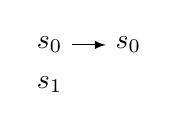
\begin{tikzpicture}[>=latex]
    \node[] (input) {$s_0$};
    \node[right of=input] (output) {$s_0$};
    \node[below of=input,node distance=.5cm] (unused) {$s_1$};
    \draw[->] (input) -- (output);
\end{tikzpicture}
\\
\begin{tikzpicture}[>=latex,node distance=.6cm]
  \node[] (input1) {$s_0$};
  \node[below of=input1] (midway) {};
  \node[below of=midway] (input2) {$s_1$};
  \node[block, right of=midway, node distance=1cm] (T) {$\lift{\pair{\cdot}{\cdot}}$};
  \draw[->] (input1) -| (T);
  \draw[->] (input2) -| (T);
  \node[block, right of=T, node distance=1.5cm] (F) {$\lift{\mbox{snd}}$};
  \node[right of=F, node distance=1cm] (output) {$s_1$};
  \draw[->] (T) -- (F);
  \draw[->] (F) -- (output);
\end{tikzpicture}
&
$\cong$
& 
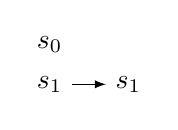
\begin{tikzpicture}[auto,>=latex]
    \node[] (input0) {$s_0$};
    \node[below of=input0,node distance=.5cm] (input1) {$s_1$};
    \node[right of=input1] (output) {$s_1$};
    \draw[->] (input1) -- (output);
\end{tikzpicture}
\\
\begin{tikzpicture}[auto,>=latex]
  \node[] (input) {$p$};
  \node[right of=input, node distance=1.5cm] (midway) {};
  \node[block, above of=midway, node distance=.5cm] (fst) {$\lift{\mbox{fst}}$};
  \node[block, below of=midway, node distance=.5cm] (snd) {$\lift{\mbox{snd}}$};
  \node[block, right of=midway, node distance=1.5cm] (q) {$\lift{\pair{\cdot}{\cdot}}$};
  \node[right of=q] (output) {$p$};
  \draw[->] (input.east) -- ++(2mm,0) |- (fst);
  \draw[->] (input.east) -- ++(2mm,0) |- (snd);
  \draw[->] (fst) -| (q);
  \draw[->] (snd) -| (q);
  \draw[->] (q) -- (output);
\end{tikzpicture} 
&
$\cong$
&
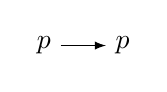
\begin{tikzpicture}[auto,>=latex]
    \node[] (input) {$p$};
    \node[right of=input] (output) {$p$};
    \draw[->] (input) -- (output);
\end{tikzpicture}
\end{tabular}
\end{center}

Pairing and projections allow for switching between pairs of streams and streams of pairs, 
whichever is more convenient. For example, instead of a binary operator 
$T:\stream{A}\times\stream{B}\to\stream{C}$ we can work with a unary operator
$T^u:\stream{A\times B}\to\stream{C}$ where $T^u(p)=T(\lift{\mbox{fst}}(p),\lift{\mbox{snd}}(p))$ 
and instead of a unary operator $Q:\stream{A\times B}\to\stream{C}$ we can work with
a binary operator $Q^b:\stream{A}\times\stream{B}\to\stream{C}$ where
$Q^b(s_0,s_1)=Q(\lift{\pair{s_0}{s_1}})$.

\begin{tabular}{m{3.5cm}m{1cm}m{5cm}}
\begin{tikzpicture}[auto,>=latex]
  \node[] (input1) {$s_0$};
  \node[below of=input1,node distance=.5cm] (midway) {};
  \node[below of=midway,node distance=.5cm] (input2) {$s_1$};
  \node[block, right of=midway] (T) {$Q^b$};
  \draw[->] (input1) -| (T);
  \draw[->] (input2) -| (T);
  \node[right of=T] (output) {$s$};
  \draw[->] (T) -- (output);
\end{tikzpicture}
&
$\defn$
& 
\begin{tikzpicture}[auto,>=latex]
  \node[] (input1) {$s_0$};
  \node[below of=input1,node distance=.5cm] (midway) {};
  \node[below of=midway,node distance=.5cm] (input2) {$s_1$};
  \node[block, right of=midway] (pair) {$\lift{\pair{\cdot}{\cdot}}$};
  \draw[->] (input1) -| (pair);
  \draw[->] (input2) -| (pair);
  \node[block, right of=pair] (T) {$Q$};
  \node[right of=T] (output) {$s$};
  \draw[->] (pair) -- (T);
  \draw[->] (T) -- (output);
\end{tikzpicture} \\

\begin{tikzpicture}[auto,>=latex]
  \node[] (input) {$p$};
  \node[block, right of=input] (Q) {$T^u$};
  \draw[->] (input) -- (Q);
  \node[right of=Q] (output) {$s$};
  \draw[->] (Q) -- (output);
\end{tikzpicture}
&
$\defn$
& 
\begin{tikzpicture}[auto,>=latex]
  \node[] (input) {$p$};
  \node[right of=input, node distance=1.5cm] (midway) {};
  \node[block, above of=midway, node distance=.5cm] (fst) {$\lift{\mbox{fst}}$};
  \node[block, below of=midway, node distance=.5cm] (snd) {$\lift{\mbox{snd}}$};
  \node[block, right of=midway] (q) {$T$};
  \node[right of=q] (output) {$s$};
  \draw[->] (input.east) -- ++(2mm,0) |- (fst);
  \draw[->] (input.east) -- ++(2mm,0) |- (snd);
  \draw[->] (fst) -| (q);
  \draw[->] (snd) -| (q);
  \draw[->] (q) -- (output);
\end{tikzpicture} 
\end{tabular}


Given two operators $Q:\stream{A}\to\stream{B}$ and $R:\stream{A}\to\stream{C}$
we define $\lift{\pair{Q}{R}}:\stream{A}\to\stream{B\times C}$ by 
$\lift{\pair{Q}{R}}(s)=\lift{\pair{Q(s)}{R(s)}}$. In terms of circuit diagrams:


\begin{tabular}{m{3.5cm}m{.5cm}m{5cm}}
\begin{tikzpicture}[auto,>=latex]
  \node[] (input) {$s$};
  \node[block, right of=input,node distance=1.5cm] (Q) {$\lift{\pair{Q}{R}}$};
  \draw[->] (input) -- (Q);
  \node[right of=Q,node distance=1.5cm] (output) {$o$};
  \draw[->] (Q) -- (output);
\end{tikzpicture}
& 
$\cong$
&
\begin{tikzpicture}[auto,>=latex,node distance=.5cm]
  \node[] (input) {$s$};
  \node[block, above right=.1cm and 1cm of input] (a) {$Q$};
  \node[block, below right=.1cm and 1cm of input] (b) {$R$};
  \node[block, right of=input, node distance=2.8cm] (P) {$\lift{\pair{\cdot}{\cdot}}$};
  \node[right of=P,node distance=1cm] (output) {$o$};
  \draw[<-] (a.west) -- ++(-5mm,0) |- (input);
  \draw[<-] (b.west) -- ++(-5mm,0) |- (input);
  \draw[->] (a) -| (P);
  \draw[->] (b) -| (P);
  \draw[->] (P) -- (output);
\end{tikzpicture}
\end{tabular}

We have standard equalities (from category theory) for this construct such
as $\lift{\mbox{fst}}\circ\lift{\pair{Q}{R}}=Q$, similarly for $\mbox{snd}$, and 
$\lift{\pair{\lift{\mbox{fst}}\circ W}{\lift{\mbox{snd}}\circ W}} = W$.
These correspond to equivalences of circuits that follow from the simpler ones above.
For example, after substituting the definition of $\pair{Q}{R}$ we have

\begin{tabular}{m{5.5cm}m{1cm}m{2.5cm}}
\begin{tikzpicture}[auto,>=latex,node distance=.5cm]
  \node[] (input) {$s$};
  \node[block, above right=.1cm and 1cm of input] (a) {$R$};
  \node[block, below right=.1cm and 1cm of input] (b) {$S$};
  \node[block, right of=input, node distance=2.8cm] (P) {$\lift{\pair{\cdot}{\cdot}}$};
  \node[block,right of=P,node distance=1.2cm] (F) {$\lift{\mbox{fst}}$};
  \node[right of=F,node distance=1cm] (output) {$o$};
  \draw[<-] (a.west) -- ++(-5mm,0) |- (input);
  \draw[<-] (b.west) -- ++(-5mm,0) |- (input);
  \draw[->] (a) -| (P);
  \draw[->] (b) -| (P);
  \draw[->] (P) -- (F);
  \draw[->] (F) -- (output);
\end{tikzpicture}
&
$\cong$
&
\begin{tikzpicture}[auto,>=latex]
    \node[] (input) {$s$};
    \node[block, right of=input,node distance=1cm] (F) {$R$};
    \node[right of=F] (output) {$o$};
    \draw[->] (input) -- (F);
    \draw[->] (F) -- (output);
\end{tikzpicture}
\end{tabular}


Another useful operator expression notation takes $Q:\stream{A}\to\stream{B}$
and $R:\stream{D}\to\stream{C}$ and combines them into
$Q\times R:\stream{A\times D}\to\stream{B\times C}$ where
$(Q\times R)(p) = \pair{Q(\lift{\mbox{fst}}(p))}{R(\lift{\mbox{snd}}(p))}$. 
This corresponds to the following circuit:

\begin{center}
\begin{tikzpicture}[auto,>=latex,node distance=.5cm]
  \node[] (input) {$p$};
  \node[block, above right=0cm and 1cm of input] (a) {$\lift{\mbox{fst}}$};
  \node[block, above right=0cm and 2.5cm of input] (Q) {$Q$};
  \node[block, below right=0cm and 1cm of input] (b) {$\lift{\mbox{snd}}$};
  \node[block, below right=0cm and 2.5cm of input] (R) {$R$};
  \node[block, right of=input, node distance=4cm] (P) {$\lift{\pair{\cdot}{\cdot}}$};
  \node[right of=P,node distance=1cm] (output) {$o$};
  \draw[<-] (a.west) -- ++(-5mm,0) |- (input);
  \draw[<-] (b.west) -- ++(-5mm,0) |- (input);
  \draw[->] (Q) -| (P);
  \draw[->] (R) -| (P);
  \draw[->] (a) -- (Q);
  \draw[->] (b) -- (R);
  \draw[->] (P) -- (output);
\end{tikzpicture}
\end{center}

We also have the following circuit equivalence:

\begin{center}
\begin{tabular}{m{3cm}m{1cm}m{2.5cm}}
\begin{tikzpicture}[auto,>=latex]
  \node[] (input) {$s$};
  \node[block, right of=input] (q) {$Q$};
  \node[above right=0cm and .5cm of q] (a) {$o_0$};
  \node[below right=0cm and .5cm of q] (b) {$o_1$};
  \draw[->] (input) -- (q);
  \draw[->] (q.east) -- ++(2mm,0) |- (a);
  \draw[->] (q.east) -- ++(2mm,0) |- (b);
\end{tikzpicture}
&
$\cong$
&
\begin{tikzpicture}[auto,>=latex]
  \node[] (input) {$s$};
  \node[block, above right=0cm and .5cm of input] (q0) {$Q$};
  \node[block, below right=0cm and .5cm of input] (q1) {$Q$};
  \node[right of=q0] (output0) {$o_0$};
  \node[right of=q1] (output1) {$o_1$};
  \draw[->] (input.east) -- ++(2mm,0) |- (q0);
  \draw[->] (input.east) -- ++(2mm,0) |- (q1);
  \draw[->] (q0) -- (output0);
  \draw[->] (q1) -- (output1);
\end{tikzpicture}
\end{tabular}
\end{center}

\val{Should this one be here? It is unrelated to products. 
Let em email you a proposal for organizing these equivalences and definitions}


Lifting functions on values and composing stream operators results in a very simple, yet limited, programming language on streams.  
We next introduce operators that ``shift'' streams in time.
These will be instrumental for enriching the language.

\subsection{Streams over abelian groups}\label{sec:abelian}

For the rest of the technical development we will require the set of values $(A, +, 0, -)$
for any stream $\stream{A}$ to form a commutative group.  

We denote by $0_{\stream{A}}$ (or simply $0$ when the type is clear) the stream that consist of the special 
value 0 at each time moment: $0_{\stream{A}} \in \stream{A}$, $\forall t \in \N . 0_{\stream{A}}[t] \defn 0_A$.

\subsubsection{Delays and time-invariance}\label{sec:delay}

\begin{definition}[Delay]
The \defined{delay operator}\footnote{The name $\zm$
comes form the DSP literature, and it is related to the z-transform.} emits an output stream that is 
the input stream delayed by one element: $\zm_A: \stream{A} \to \stream{A}$ defined by:
$$
\zm_A(s)[t] \defn  \begin{cases}
s[t - 1] & \text{when}~t\geq1\\
0_A      & \text{when}~t=0
\end{cases}
$$

We often omit the type parameter $A$, and write just $\zm$.
We denote by $z^{-k}$ the composition of $\zm$
with itself $k$ times (delay by $k$ time units). 
\end{definition}

\begin{center}
\begin{tikzpicture}[auto,node distance=1cm,>=latex]
    \node[] (input) {$i$};
    \node[block, right of=input] (z) {$\zm$};
    \node[right of=z] (output) {$o$};
    \draw[->] (input) -- (z);
    \draw[->] (z) -- (output);
\end{tikzpicture}
\end{center}

For example, the delay of the $\id$ stream is $\zm(\id)$, containing
the sequence of values $\sv{0 0 1 2 3}$.

\qquad

The following definition applies to stream operators of
any number of arguments but to keep the notation simpler we formulate it only for binary operators.

\begin{definition}[Time invariance]
A stream operator $T: \stream{A_0}\times\stream{A_1} \to \stream{B}$ is \defined{time-invariant} if it commutes with the delay operator $\zm$, that is, \\
$T(\zm(s_0),\zm(s_1)) = \zm(T(s_0,s_1))$ for any $s_0 \in \stream{A_0}, s_1 \in \stream{A_1}$.
\end{definition}
In other words, $T$ is time-invariant if and only if the following two circuits are equivalent:

\begin{center}
\begin{tabular}{m{3cm}m{.5cm}m{3cm}}
\begin{tikzpicture}[auto,node distance=.5cm,>=latex]
  \node[] (input1) {$s_0$};
  \node[below of=input1] (midway) {};
  \node[below of=midway] (input2) {$s_1$};
  \node[block, right of=midway, node distance=1cm] (T) {$T$};
  \node[block, right of=T,node distance=1cm] (z) {$\zm$};
  \node[right of=z,node distance=1cm] (output) {$o$};
  \draw[->] (input1) -| (T);
  \draw[->] (input2) -| (T);
  \draw[->] (T) -- (z);
  \draw[->] (z) -- (output);
\end{tikzpicture}
&
$\cong$
&
\begin{tikzpicture}[auto,node distance=.5cm,>=latex]
  \node[] (input1) {$s_0$};
  \node[below of=input1] (midway) {};
  \node[below of=midway] (input2) {$s_1$};
  \node[block, right of=input1, node distance=1cm] (z1) {$\zm$};
  \node[block, right of=input2, node distance=1cm] (z2) {$\zm$};
  \node[block, right of=midway, node distance=2cm] (T) {$T$};
  \node[right of=T,node distance=1cm] (output) {$o$};
  \draw[->] (input1) -- (z1);
  \draw[->] (input2) -- (z2);
  \draw[->] (z1) -| (T);
  \draw[->] (z2) -| (T);
  \draw[->] (T) -- (output);
\end{tikzpicture}
\end{tabular}
\end{center}

It is straightforward to check that the composition
of any number of time-invariant operators of any number of arguments
is time invariant. Similarly, the delay operators $z^{-k}$ as well as the
pairing and projection operators are time-invariant. 
In this framework we only deal with time-invariant operators.

\begin{definition}
We say that a function between groups $f: A \to B$ has the \defined{zero-preservation
property} iff $f(0_A) = 0_B$.  We write $\zpp{f}$.  This property generalizes to functions
with multiple inputs: e.g., $g: A \times B \to C$ where $A, B, C$ are groups.  $\zpp{g}$ 
iff $g(0_A, 0_B) = 0_C$.
\end{definition}

\begin{proposition}
A lifted operator $\lift{f}$ is time-invariant iff $\zpp{f}$. 
\end{proposition}

Notice that it is easy to construct operators that are not time-invariant.
Consider the ``constant 1'' function: $c_1: \N \rightarrow \N$, defined by 
$c_1(x) = 1, \forall x \in \N$.
The stream operator defined by $\lift{c_1}: \stream{N} \rightarrow \stream{N}$ 
produces a stream containing only the constant value 1: $c_1(s)[t] = 1, 
\forall s \in \stream{N}, t \in \N$.  The stream operator $\lift{c_1}$
is \emph{not} time-invariant, since it does not have the zero preservation property.

\begin{comment}
\begin{definition}
We call an operator $o: \stream{A} \rightarrow \stream{B}$ over streams 
\defined{memoryless} if it can be produced by lifting a function pointwise, i.e., 
there exists a function $f: A \rightarrow B$ such that 
$\forall s \in \stream{A} . o(s)[t] = f(s[t])$.

\begin{example}
Whatever definition we give to ``memoryless'' it should be the case that 
any memoryless operator is causal. 
\end{example}
\end{definition}
\end{comment}

\subsection{Causal and strict operators}\label{sec:causal}

For notation simplicity we again give the next definition only for unary operators;
it extends naturally to binary operators through the use of pairing as shown above.

\begin{definition}[Causality]
A stream operator, $S:\stream{A}\to\stream{B}$,
is \defined{causal} when for any $s,s'\in\stream{A}$,
and all times $t$ we have 
$$
(\forall i\leq t~s[i]=s'[i]) ~~\text{implies}~~ S(s)[t]=S(s')[t]
$$
\end{definition}

Note that all operators produced by lifting scalar functions are causal. 
$\zm$ is causal.  All \dbsp operators are causal.

\begin{definition}[Cutting]
\defined{Cutting} the stream $s \in \stream{A}$ at time $t \in \N$ produces a stream
$$
(\cut{s}{t})[i] \defn  \begin{cases}
                      s[i] &\text{if}~i\leq t\\
                      0_A  &\text{if}~i>t
                      \end{cases}
$$
\end{definition}
For example, cutting the stream $\id$ at time 2 gives the stream $\cut{\id}{2}$
composed of the sequence $\sv{0 1 2 0 0}$.

Note that $\cut{\cut{s}{t_1}}{t_2}=\cut{s}{\min(t_1,t_2)}$. It follows that
$\cut{\cut{s}{t_1}}{t_2}=\cut{\cut{s}{t_2}}{t_1}$ (cutting is commutative) and
$\cut{\cut{s}{t}}{t}=\cut{s}{t}$, (cutting at time $t$ is idempotent).
Cutting, however, is \textbf{not} time-invariant.  Cutting is not 
used as a \dbsp operator, it is just a mathematical tool that we will use to 
reason about the behavior of the circuits we build.

\begin{lemma}
\label{lemma-causal-characterization}
The following are equivalent for a binary stream operator $T$
\begin{enumerate}
\item[(i)] $T$ is causal
\item[(ii)] $\forall s_1,s_2$ and $t$  we have $\cut{T(s_1,s_2)}{t} ~=~ \cut{T(\cut{s_1}{t},\cut{s_2}{t})}{t}$~.
\end{enumerate}
\end{lemma}
Using part (ii) it follows immediately that the composition
of any number of causal operators of any number of arguments is causal.
Moreover, using also the commutativity and idempotence of cutting, it follows that
for any $t$ the operator $\lambda s.\cut{s}{t}$ is itself causal.

\begin{definition}[zero almost everywhere]\label{def:zae}
We say that a stream $s$ is \defined{zero almost-everywhere} if there exists a time $t_0 \in \N$
s.t. $\cut{s}{t_0} = s$.
\end{definition}

%Such a stream can be described entirely by providing its prefix up to time $t_0$,
%a finite stream.  
We denote the set of streams over $A$ that are zero almost everywhere
by $\streamf{A}$.

\begin{definition}[Strictness]
A stream operator, $F:\stream{A}\to\stream{B}$
is \defined{strictly causal} (abbreviated \textbf{strict})
if for any $s,s'\in\stream{A}$ and all times $t$ we have 
$$
(\forall i<t . s[i]=s'[i]) ~~\text{implies}~~ F(s)[t]=F(s')[t]
$$
\end{definition}

In particular, $F(s)[0] = 0_B$ is the same for all inputs $s \in \stream{A}$.
Strict operators are of course causal. Note that lifted stream operators,
while causal, in general are \emph{not} strict. 

It can be immediately checked that the operator $\zm$ 
(in fact, $z^{-k}$ for any positive integer $k$)  
is strict. 
In this text $\zm$ is the only primitive strict operator used.

\begin{definition}[Strict cutting]
\defined{Strictly cutting} the stream $s \in \stream{A}$ at time $t \in \N$ produces the stream
$$
(\scut{s}{t})[i] \defn  \begin{cases}
                      s[i] &\text{if}~i< t\\
                      0_A  &\text{if}~i\geq t
                      \end{cases}
$$
\end{definition}

$\scut{s}{0}$ is the stream $0_{\stream{A}}$ that is $0_A$ at all times.
Note also that $\scut{s}{t+1} =\cut{s}{t}$.


Analogously to Lemma~\ref{lemma-causal-characterization} an operator $F: \stream{A} \to \stream{B}$ is strict iff for any $s$ and $t$ we have
$$
\cut{F(s)}{t} ~=~ \cut{F(\scut{s}{t})}{t}
$$
In particular, $F(s)[0] = F(0_{\stream{A}})[0]$ and
$F(s)[t+1]=F(\cut{s}{t})[t+1]$.  Note the different zeros in $F(0_{\stream{A}})[0]$: 
it features both the stream $0_{\stream{A}} \in \stream{A}$, consisting of the group element $0_A$ 
at each time moment, and the time moment $0$.

The next proposition shows the importance of strict operators.
\begin{proposition}
\label{prop-unique-fix}
For any strict operator $F: \stream{A} \to \stream{A}$ the equation ~$\alpha=F(\alpha)$~ has a unique
solution $\alpha \in \stream{A}$.  In other words, every strict operator has a unique fixed point,
which we denote by $\fix{\alpha}{F(\alpha)}$.
\end{proposition}
%\leonid{Usually fixed-points require some monotonicity.  What is it here?}

\begin{proof}
Define the solution (the fixed point) by recurrence:
\begin{eqnarray*}
\alpha[0] & = &  F(\alpha)[0]=F(0_{\stream{A}})[0]\\
\alpha[t+1] & = & F(\alpha)[t+1]=F(\cut{\alpha}{t})[t+1]
\end{eqnarray*}
The second equality defines $\alpha[t+1]$ in terms of $\alpha[0],\ldots,\alpha[t]$.
Uniqueness follows by strong induction.

\qquad
\end{proof}

We will apply the previous proposition to operators obtained by composing strict and causal ones.
\begin{lemma} 
\label{lemma-causal-strict}
Let $k\geq 2$. If $F$ is strict and the $k$-ary $T$ operator is causal, then for any 
fixed $s_0,\ldots,s_{k-2}$ the operator
$\lambda\alpha.T(s_0,\ldots,s_{k-2},F(\alpha))$ is strict. 
\end{lemma}

\begin{proof} We show the case $k=2$.
This operator is described by the following diagram with a ``feedback loop'':

\begin{center}
\begin{tikzpicture}[>=latex]
    \node[] (input) {$s$};
    \node[block, right of=input] (f) {$T$};
    \node[right of=f, node distance=1.5cm] (output) {$\alpha$};
    \node[block, below of=f, node distance=.8cm] (z) {$F$};
    \draw[->] (input) -- (f);
    \draw[->] (f) -- node (mid) {} (output);
    \draw[->] (mid.center) |-  (z);
    \draw[->] (z.west) -- ++(-.3,0) |- ([yshift=1mm]f.south west);
\end{tikzpicture}
\end{center}
\begin{eqnarray*}
\cut{T(s,F(\alpha))}{t} & = & \cut{T(\cut{s}{t},\cut{F(\alpha)}{t})}{t}\\
                   & = & \cut{T(\cut{s}{t},\cut{F(\scut{\alpha}{t})}{t})}{t}\\
                   & = & \cut{T(s,F(\scut{\alpha}{t}))}{t}
\end{eqnarray*}
\qquad
\end{proof}


\begin{corollary} 
\label{cor-fix-cut}
For strict $F$ we have
$$
\cut{(\fix{\alpha}{F(\alpha)})}{t} ~=~  \fix{\alpha}{(\cut{F(\alpha)}{t})}
$$
\end{corollary}
\begin{proof}
Since cutting itself is a causal operator, it follows from Lemma~\ref{lemma-causal-strict} that $\lambda\alpha.(\cut{F(\alpha)}{t})$ is strict
so Proposition~\ref{prop-unique-fix} applies and $\fix{\alpha}{(\cut{F(\alpha)}{t})}$
is well-defined.

If we let $\alpha$ be the solution of $\alpha=F(\alpha)$ then, by uniqueness, it suffices to show that $\beta=\cut{\alpha}{t}$ satisfies 
the equation $\beta=\cut{F(\beta)}{t}$. Indeed, since $F$ is in particular causal
$$
\cut{\alpha}{t} = \cut{F(\alpha)}{t} = \cut{F(\cut{\alpha}{t})}{t}
$$


\qquad
\end{proof}

\begin{corollary}\label{feedback-semantics}
\label{cor-loop}
Let $k\geq1$. If $F: \stream{A} \to \stream{A}$ is strict and $(k+1)$-ary $T$ is causal then the $k$-ary
operator $Q(s_0,\ldots,s_{k-1})=\fix{\alpha}{T(s_0,\ldots,s_{k-1},F(\alpha))}$~ is well-defined and causal. 
If, moreover, $F$ and $T$ are time-invariant then so is $Q$.
\end{corollary}
\begin{proof} We show the case $k=1$.
The well-definedness of $Q$ follows by applying, for each $s$, Proposition~\ref{prop-unique-fix}
to the operator
$\lambda\alpha.T(s,F(\alpha))$ which is strict by Lemma~\ref{lemma-causal-strict}.
For future reference it might be useful to state the defining recurrence for a stream $\alpha$ 
produced by this operator, that is, $\alpha=Q(s)$:
\begin{eqnarray*}
\alpha[0] & = &  T(s,F(0_{\stream{A}}))[0]\\
\alpha[t+1] & = & T(s,F(\cut{\alpha}{t}))[t+1]
\end{eqnarray*}
To prove that $Q$ is causal we could use this recurrence and induction. Instead 
we use the causality of $T$ and the idempotence of cutting in conjunction with
Corollary~\ref{cor-fix-cut} as follows:
\begin{eqnarray*}
\cut{Q(s)}{t} & = &  \cut{(\fix{\alpha}{T(s,F(\alpha))})}{t}\\
         & = &  \fix{\alpha}{\cut{(T(s,F(\alpha))}{t})}~~~~~~~~~~~~\mbox{(Corollary~\ref{cor-fix-cut})}\\
         & = &  \fix{\alpha}{(\cut{T(\cut{s}{t},\cut{F(\alpha)}{t})}{t})}~~~~~~\mbox{(Causality of $T$)}\\
         & = &  \fix{\alpha}{(\cut{T(\cut{\cut{s}{t}}{t},\cut{F(\alpha)}{t})}{t})}~~~\mbox{(Idempotence of cutting)}\\
         & = &  \fix{\alpha}{\cut{(T(\cut{s}{t},F(\alpha))}{t})}~~~~~~~~~~\mbox{(Causality of $T$)}\\
         & = & \cut{(\fix{\alpha}{T(\cut{s}{t},F(\alpha))})}{t}~~~~~~~~~~\mbox{(Corollary~\ref{cor-fix-cut})}\\
         & = & \cut{Q(\cut{s}{t})}{t}
\end{eqnarray*}
For time-invariance we observe that if $\alpha=T(s,F(\alpha))$ then $\zm(\alpha)= \zm(T(s,F(\alpha)))=T(\zm(s),\zm(F(\alpha))= 
T(\zm(s),F(\zm(\alpha)))$. It follows that $\beta=\zm(\alpha)$ satisfies the equation $\beta=T(\zm(s),F(\beta))$ so, 
by uniqueness of the fixed point $Q(\zm(s))=\zm(Q(s))$.
\end{proof}



Ostensibly this covers a form of straightforward recursion but how about mutual recursion? For instance, assuming $T_1,T_2$ are causal and $F_1,F_2$ are strict we wish to claim that the following is well defined: $Q_1(s_1,s_2)=\alpha_1$ and $Q_2(s_1,s_2)=\alpha_2$ where:
\begin{eqnarray*}
\alpha_1 & = & T_1(s_1,F_1(\alpha_2))~~~~~\mbox{and}\\
\alpha_2 & = & T_2(s_2,F_2(\alpha_1))
\end{eqnarray*}
Here is the corresponding diagram:

\begin{tikzpicture}[>=latex]
  \node[] (i1) {$s_1$};
  \node[below of=i1, node distance=.7cm] (i2) {$s_2$};
  \node[block, right of=i1, node distance=1.5cm] (t1) {$T_1$};
  \node[block, right of=i2, node distance=1.5cm] (t2) {$T_2$};
  \node[right of=t1, node distance=1.5cm] (o1) {$\alpha_1$};
  \node[right of=t2, node distance=2cm] (o2) {$\alpha_2$};
  
  \node[block, below of=t2] (f1) {$F_2$};
  \node[block, below of=f1, node distance=.7cm] (f2) {$F_1$};
  
  \draw[->] (i1) -- (t1);
  \draw[->] (i2) -- (t2);
  \draw[->] (t1) -- node (m1) {} (o1);
  \draw[->] (t2) -- node (m2) {} (o2);
  \draw[->] (m1.center) |- (f1);
  \draw[->] (m2.center) |- (f2);
  
  \draw[->] (f1.west) -- ++(-.3,0) |- ([yshift=1mm]t2.south west);
  \draw[->] (f2.west) -- ++(-.4,0) |- ([yshift=1mm]t1.south west);
  
\end{tikzpicture}

In section~\ref{sec:pairing} we defined constructions on pairs of streams/streams of pairs. 
%that we defined in Section~\ref{sec:cartesian} 
In particular, for binary $T_1:\stream{A_1}\times\stream{B_1}\to\stream{C_1}$ and 
binary $T_2:\stream{A_2}\times\stream{B_2}\to\stream{C_2}$ 
let
\val{For binary operators we should have defined $\times$ this way in section~\ref{sec:pairing} ...
Also, in the def of $T_1\times T_2$ note that I did not put a lift in front of the stream pairing operator on the RHS. }
binary $T_1\times T_2:\stream{A_1\times A_2}\times\stream{B_1\times B_2}\to\stream{C_1\times C_2}$ 
$$
[T_1\times T_2](p,q) = \pair{T_1(\lift{\mbox{fst}}\circ p,\lift{\mbox{fst}}\circ q)}
{T_2(\lift{\mbox{snd}}\circ p,\lift{\mbox{snd}}\circ q)}
$$
In addition, we use $F_1\times F_2:\stream{C_1\times C_2}\to\stream{B_1\times B_2}$ as defined in section~\ref{sec:pairing}. Let also $\mbox{swap}: C_1\times C_2 \to C_2 \times C_1$
be the operator that swaps the components of a pairs (obtained by pairing the second projection
with the third.
\begin{proposition}
If $T_1$ and $T_2$ are causal then $T_1\circ T_2$ is causal. If $F_1$ and $F_2$ are strict then
$(F_1\times F_2)\circ\lift{\mbox{swap}}$ is strict.
\end{proposition}
The circuit above is equivalent to the following (when composed with projections of outputs
and pairing of inputs:

\begin{tikzpicture}[>=latex]
    \node[] (input) {$s$};
    \node[block, right of=input, node distance=2cm] (f) {$T_1\times T_2$};
    \node[right of=f, node distance=3cm] (output) {$\alpha$};
    \node[block, below of=f] (z) {($F_1\times F_2)\circ\lift{\mbox{swap}}$};
    \draw[->] (input) -- (f);
    \draw[->] (f) -- ++(2,0) node (mid) {} -- (output);
    \draw[->] (mid.center) |-  (z);
    \draw[->] (z.west) -- ++(-.3,0) |- ([yshift=1mm]f.south west);
\end{tikzpicture}


In other words, 
we can apply Corollary~\ref{feedback-semantics} to the causal operator $T_1\times T_2$
and the strict operator $F_1\times F_2$ and obtain $Q_1$ and $Q_2$ from
$$
\fix{\alpha}{[T_1\times T_2](\pair{s_1}{s_2},[F_1\times F_2](\mbox{swap}(\alpha)))}
$$
by further projecting, where $\alpha$ is a variable of type pair of streams and $\overline{\alpha}$
swaps the two components.





\val{We should state this a some kind of corollary to the corollary.}
\mihai{This becomes complicated for $n$-way mutual recursion, you have a quadratic number of edges.
Maybe it's simpler to assume that all of them use all of the alphas, and the projection to a subset
is part of $T$ if needed.}



\subsection{Streams as an abelian group}\label{sec:abelianstreams}

Remember that we require the elements of a stream to come from an Abelian group:
$(A,+,0,-)$.  This structure also lifts to streams:

\begin{proposition}
$(\stream{A},+,0_{\stream{A}},-)$ (with the operations lifted pointwise in time) 
is also an abelian group. Moreover, lifting a group homomorphism produces
a stream operator that is itself a group homomorphism.
In addition, when $A$ and $B$ are abelian groups there is a standard abelian group structure
on $A\times B$, with the zero $0_{A \times B}$ the pair $\pair{0_A}{0_B}$.
\end{proposition}


\begin{definition}[linear]
If $A$ and $B$ are abelian groups, we call
a function $f: A \rightarrow B$ \defined{linear} if it is a group homomorphism, that is,
$f(a+b)=f(a)+f(b)$ (and therefore $f(0_A)=0_B$ and $f(-a)=-f(a)$); thus $\zpp{f}$.
\end{definition}

We use the abbreviation LTI for a stream operator that is linear and time-invariant.

Lifting a linear function $f: A \to B$ produces a stream operator $\lift{f}$ that is causal and LTI. 
It follows that stream addition and negation are causal and LTI.
$\zm$ is LTI, (and so is $z^{-k}$ for all $k$).

\begin{definition}[multilinear, bilinear]
We define \defined{multilinear} (in particular, \defined{bilinear}) functions as functions (between groups) of multiple
arguments that are linear separately in each argument (that is, if we fix all but one argument,
the resulting function is linear in that argument.  In other words, the function distributes over addition): 
e.g., for $g: A_0 \times A_1 \to B, \forall a, b \in A_0, c, d \in A_1 . g(a+b, c) = g(a, c) + g(b, c)$, 
and $g(a, c+d) = g(a, c) + g(c, d)$.
\end{definition}

Multiplication over $\Z$ is a bilinear function.  For a bilinear function $g$ we have $\zpp{g}$.

This definition extends to stream operators.
Lifting any bilinear function $g: A \times B \to C$ produces a bilinear stream operator $\lift{g}$.
An example bi-linear operator over $\stream{\Z}$ is the lifted integer multiplication: 
$T: \stream{\Z} \times \stream{\Z} \to \stream{\Z}, T(a, b)[t] = a[t]\cdot b[t]$.

The composition of multilinear operators with linear operators is multilinear (since homomorphisms compose).
Since linear and bilinear functions have the zero-preservation property,
lifted linear and bilinear functions operators are all time-invariant.

\begin{proposition}
The composition of a bilinear operator followed by a linear operator is a bilinear operator.
\end{proposition}
\begin{proof}
Consider $T: \stream{A} \times \stream{B} \to \stream{C}$ a bilinear operator, and 
$S: \stream{C} \to \stream{C}$, a linear operator.  Let us compute $S(T(a+b, c)) = S(T(a, c) + T(b, c)) = 
S(T(a, c)) + S(T(b, c)).$  Thus $S \circ T$ is bilinear.
\end{proof}

Lifting a multilinear operator $A_1\times\cdots\times A_n \rightarrow B$ produces a multilinear, time-invariant stream operator. Although combining pairs (tuples) of 
streams into stream of pairs (tuples) can be useful
we must note a distinction (well understood in algebra): 
we have seen that we can use instead of a binary stream operator
$T:\stream{A}\times\stream{B}\to\stream{C}$ a unary version that acts on streams of pairs
$T^u:\stream{A\times B}\to\stream{C}$ where $T^u\pair{a}{b}=T(a,b)$. However, in contrast to causality,
there is, in general, no relation between the linearity. %\footnote{Recall the
%abelian group structure on $A\times B$.} of $T^u$ and the bilinearity of $T$. 
%\mihai{I still think that the motivation for this statement is unclear.}

In traditional signal processing most operators are LTI but in our development
we will use some important non-linear ones. 

The ``feedback-loop'' operators defined by recurrence in Corollary~\ref{cor-loop},
e.g., $\lambda s.\fix{\alpha}{T(s,F(\alpha))}$ are, in general, not (multi)linear.
\val{Counterexample even for bilinear $S$ and $\lambda s_1.\lambda s_2.\fix{\alpha}{S(s_1,s_2+\zm(\alpha))}$? Possibly $S$ is join NOT followed by distinct?}
However, multilinearity holds in important particular cases,
as shown in the following proposition:

\begin{proposition}
\label{prop-rec-linear}
Let $S$ be a unary causal, LTI operator. Then, the
operator $Q(s)=\fix{\alpha}{S(s+\zm(\alpha))}$~ is well-defined and LTI.
\end{proposition}
\mihai{Notice that this is a very nice kind of recursion, a tail-recursion.}

\begin{center}
\begin{tikzpicture}[>=latex]
    \node[] (input) {$s$};
    \node[block, shape=circle, right of=input, inner sep=0pt] (plus) {$+$};
    \node[block, right of=plus] (Q) {$S$};
    \node[right of=Q, node distance=1.5cm] (output) {$\alpha$};
    \node[block, below of=Q, node distance=.8cm] (z) {$\zm$};
    \draw[->] (input) -- (plus);
    \draw[->] (plus) -- (Q);
    \draw[->] (Q) -- node (mid) {} (output);
    \draw[->] (mid.center) |-  (z);
    \draw[->] (z) -| (plus);
\end{tikzpicture}
\end{center}

\begin{proof} Since $S$ and the addition operator
are causal and $\zm$ is strict, Proposition~\ref{prop-unique-fix} applies, 
for each $s$, to the operator
$\lambda\alpha.S(s+\zm(\alpha))$ which is strict by Lemma~\ref{lemma-causal-strict}.
Thus $Q$ is well-defined.

Fix streams $s_0$ and $s_1$. Let $\alpha_0$
be the unique solution of $\alpha_0=S(s_0+\zm(\alpha_0))$ and 
$\alpha_1$ be the unique solution of $\alpha_1=S(s_1+\zm(\alpha_1))$.
Then $\alpha=\alpha_0+\alpha_1$ is the unique solution of 
$\alpha=Q(s_0+s_1+\zm(\alpha))$. This is justified by adding the equations
and using the linearity of $S$ and the linearity of $\zm$.
\end{proof}

\begin{proposition}
If $T$ is binary causal, $G$ is unary causal, and $F$ is unary strict then:
$$
\fix{\alpha}{G(T(s,F(\alpha)))} = G(\fix{\beta}{T(s,F(G(\beta)))})
$$

\noindent In terms of diagrams:

\begin{tabular}{m{4cm}m{1cm}m{5cm}}
\begin{tikzpicture}[>=latex]
    \node[] (input) {$s$};
    \node[block, right of=input] (t) {$T$};
    \node[block, right of=t] (g) {$G$};
    \node[right of=g, node distance=1.5cm] (output) {$o$};
    \node[block, below of=t, node distance=.8cm] (f) {$F$};
    \draw[->] (input) -- (t);
    \draw[->] (t) -- (g);
    \draw[->] (g) -- node (mid) {} (output);
    \draw[->] (mid.center) |-  (f);
    \draw[->] (f.west) -- ++(-.3,0) |- ([yshift=1mm]t.south west);
\end{tikzpicture}
&
$\cong$
&
\begin{tikzpicture}[>=latex]
    \node[] (input) {$s$};
    \node[block, right of=input, node distance=2cm] (t) {$T$};
    \node[block, right of=t, node distance=1.5cm] (g) {$G$};
    \node[right of=g] (output) {$o$};
    \node[block, below of=t, node distance=.8cm] (g1) {$G$};
    \node[block, left of=g1] (f) {$F$};
    \draw[->] (input) -- (t);
    \draw[->] (t) -- node (mid) {} (g);
    \draw[->] (g) -- (output);
    \draw[->] (mid.center) |-  (g1);
    \draw[->] (g1) -- (f);
    \draw[->] (f.west) -- ++(-.3,0) |- ([yshift=1mm]t.south west);
\end{tikzpicture}
\end{tabular}
\end{proposition}

\begin{proof}
For the second fixpoint to exist we need to show that $F\circ G$ is strict.
Once we do that, by uniqueness of solutions, it remains to show that if $\beta$ is a solution to  $\beta=T(s,F(G(\beta))$ then $\alpha=G(\beta)$ is a solution to
$\alpha=G(T(s,F(\alpha))$ which is immediate by applying $G$ to the first equation.
So let's prove that $F\circ G$ is strict. For $t>0$ we have
\begin{eqnarray*}
\cut{F(G(s))}{t} & = & \cut{F(\scut{G(s)}{t})}{t}~~~~~\mbox{($F$ strict)}\\
                 & = & \cut{F(\cut{G(s)}{t-1})}{t}~~~~~\mbox{($t\geq1$)}\\
                 & = & \cut{F(G(\cut{s}{t-1}))}{t}~~~~~\mbox{($G$ causal)}\\ 
                 & = & \cut{F(G(\scut{s}{t}))}{t}
\end{eqnarray*}
For $t=0$ just observe that $F(G(s))[0]$ is the same for any $G(s)$ therefore for any $s$.
Note that if $G$ is not causal then $F\circ G$ is not strict and the fixed point may not exist.
\end{proof}


\subsection{Differentiation and Integration}

\begin{definition}[Differentiation]
The \defined{differentiation operator} $\D_{\stream{A}} : \stream{A} \to \stream{A}$ is defined by:
$$
\D_{\stream{A}}(s) \defn s - \zm(s)
$$ 
\end{definition}
We generally omit the type, and write just $\D$ when the type can be inferred from the context.

The value of $\D(s)$ (at time $t$) is the difference
between  the current (time $t$) value of $s$ and the previous (time $t-1$) value of $s$.

As an example, applying $\D$ to the stream $\id$ gives a result a
stream $\D(\id)$ containing the values $\sv{0 1 1 1 1}$.

\begin{center}
\begin{tikzpicture}[auto,>=latex,node distance=1cm]
    \node[] (input) {$s$};
    \node[block, shape=circle, right of=input, inner sep=0pt,node distance=2cm] (plus) {$+$};
    \node[right of=plus] (output) {$\D(s)$};
    \draw[draw,->] (input) -- node (i) {} (plus);
    \node[block, below of=i, node distance=.8cm] (z) {$\zm$};
    \node[block, shape=circle, right of=z, inner sep=0pt] (minus) {$-$};
    \draw[->] (plus) -- (output);
    \draw[->] (i) -- (z);
    \draw[->] (z) -- (minus);
    \draw[->] (minus) -- (plus);
\end{tikzpicture}
\end{center}

\begin{proposition}
\label{prop-diff-properties}
The differentiation operator $\D$ is causal and LTI.
\end{proposition}
\begin{proof}
Follow from definition using the properties of subtraction and delay.
\end{proof}

The integration operator ``reconstitutes'' a stream from its changes:

\begin{definition}[Integration]
The \defined{integration operator}  $\I_{\stream{A}} : \stream{A} \to \stream{A}$ 
is defined by $\I_{\stream{A}}(s) \defn \lambda s . \fix{\alpha}{(s + \zm(\alpha))}$.
\end{definition}

\noindent
We also generally omit the type, and write just $\I$.
This is the construction from Proposition~\ref{prop-rec-linear} 
using the identity function for $S$.

\begin{center}
\begin{tikzpicture}[auto,>=latex]
    \node[] (input) {$s$};
    \node[block, shape=circle, right of=input, inner sep=0pt] (plus) {$+$};
    \node[right of=plus, node distance=2cm] (output) {$\I(s)$};
    \node[block, below of=plus, node distance=.8cm] (z) {$z^{-1}$};
    \draw[draw,->] (input) -- (plus);
    \draw[->] (plus) -- node (o) {} (output);
    \draw[->] (o) |- (z);
    \draw[->] (z) -- (plus);
\end{tikzpicture}
\end{center}

As an example, applying $\I$ to the $\id$ stream gives as result
a stream $\I(\id)$ composed of the values $\sv{0 1 3 6 10}$.

\begin{proposition}~\label{iprop}
$\I(s)$ is the discrete (indefinite) integral applied to the stream $s$: 
$\I(s)[t] = \sum_{i \leq t} s[i]$.
\end{proposition}
\begin{proof} The recurrence from Corollary~\ref{cor-loop} specializes to
\begin{eqnarray*}
\alpha[0]  & = & s[0]\\
\alpha[t+1] & = & \alpha[t] + s[t+1]
\end{eqnarray*}
and it's straightforward to check that $\alpha[t]= \sum_{i \leq t} s[i]$ satisfies 
it.
\end{proof}

\begin{proposition}[Properties of $\I$] 
\label{prop-integ-properties}
The integration operator $\I$ is causal and LTI.
\end{proposition}
\begin{proof}
By Proposition~\ref{iprop} these properties follow from Corollary~\ref{cor-loop} and Proposition~\ref{prop-rec-linear}.  They also be checked directly using
the definition by summation.
\end{proof}


\begin{theorem}[Inversion]
\label{inverses}
The integration and differentiation operators are inverse to each other. Equivalently, for any streams 
$\alpha$ and $s$ we have $\alpha=\I(s)$ iff $\D(\alpha)=s$.
\end{theorem}
\begin{proof}
This can be shown directly from the definitions, for example
  $$
  \begin{aligned}
  \D(\I(s))[t] &= (\I(s) - \zm(\I(s)))[t] & \mbox{definition of }\D \\
  &= \sum_{k \leq t} s[k] - \zm(\sum_{k \leq t} s[k])[t] &
  \mbox{Property }~\ref{prop-integ-properties} \\
  &= \sum_{k \leq t} s[k] - \sum_{k \leq t-1} s[k] & \mbox{definition of }\zm \\
  &= s[t]
  \end{aligned}
  $$
(and similarly we can show that $\I(\D(s'))[t] =s'[t]$).
  
Alternatively, the equivalent form of the theorem follows from Proposition~\ref{iprop} by observing that
$\D(\alpha)=s$ iff $\alpha=s+\zm(\alpha)$ which is the equation on streams that defines $\alpha=\I(s)$.
%A third proof, bringing some new insights, is given in Section~\ref{sec:ztransform}.
\end{proof}

So we have the following circuit equivalence:

\noindent
\begin{tabular}{m{3.5cm}m{.7cm}m{1.5cm}m{.7cm}m{3.5cm}}
\begin{tikzpicture}[auto,>=latex]
    \node[] (input) {$s$};
    \node[block, right of=input] (I) {$\I$};
    \node[block, right of=I] (D) {$\D$};
    \node[right of=D] (output) {$o$};
    \draw[->] (input) -- (I);
    \draw[->] (I) -- (D);
    \draw[->] (D) -- (output);
\end{tikzpicture}
     &  
     $\cong$
     &
\begin{tikzpicture}[auto,>=latex]
    \node[] (input) {$s$};
    \node[right of=input] (output) {$o$};
    \draw[->] (input) -- (output);
\end{tikzpicture}
     &
     $\cong$
     &
\begin{tikzpicture}[auto,>=latex]
    \node[] (input) {$s$};
    \node[block, right of=input] (D) {$\D$};
    \node[block, right of=D] (I) {$\I$};
    \node[right of=I] (output) {$o$};
    \draw[->] (input) -- (D);
    \draw[->] (D) -- (I);
    \draw[->] (I) -- (output);
\end{tikzpicture}
\end{tabular}


Since $\I$ and $\D$ are inverse to each other they are both bijections on streams.

If we define addition of pairs as adding the pair elements pointwise, we also have
the following identities: $\I(\pair{s}{t}) = \pair{\I(s)}{\I(t)}$ and $\D(\pair{s}{t}) = \pair{\D(s)}{\D(t)}$.

\paragraph{Observation}
It is a standard algebraic fact that the inverse of a homomorphism is also a homomorphism. 
Thus, $\I$ is linear iff $\D$ is linear. Another immediate consequence of this theorem is that $\I$ is time-invariant iff
$\D$ is time-invariant. 
%\val{I believe but I have not checked that}
%\mihai{It looks right}
Moreover $\I$ is causal iff
$\D$ is causal. Therefore by the Inversion Theorem we could have stated and proved only one of Proposition~\ref{prop-integ-properties} or
Proposition~\ref{prop-diff-properties}.


\paragraph{Observation} In digital signal processing, $\I$ is a IIR, an infinite-impulse response filter: given a cut stream it can produce an unbounded stream.  $\D$ is a FIR, a finite-impulse response filter: from a cut stream it always produces a cut stream.


\begin{comment}
\begin{lemma}
  The operators $\I$ and $\D$ are linear.
\end{lemma}
\begin{proof}
  $\D$ is the composition of three linear 
  operators.Let us prove the statement for $\I$.
  $$
\begin{aligned}
  (\I(a + b))[t] &= \sum_{k \leq t}(a + b)[t] & \mbox{ definition of }\D \\
  &= \sum_{k \leq t} a[k] + \sum_{k \leq t} b[k] & \mbox{ commutativity, linearity of + } \\
  &= \I(a)[t] + \I(b)[t] & \mbox{ definition of }\I.
\end{aligned}
$$

An alternative proof: using the linearity of $\zm$ we can show 
that $\alpha=\I(a)+\I(b)$ satisfies $\alpha = \zm(\alpha) + a+b$.
It follows that $\alpha=\I(a+b)$.
\end{proof}

By substituting $a + b$ with $a + (-b)$ we obtain that $\I(a - b) = \I(a) - \I(b)$, 
$\D(a - b) = \D(a) - \D(b)$ and $\zm(a - b) = \zm(a) - \zm(b)$.
\end{comment}

\section{Incremental computation}\label{sec:incremental}

\begin{definition}
Given a unary stream operator $Q: \stream{A} \to \stream{B}$ we define the 
\defined{incremental version} of $Q$ as $\inc{Q} \defn \D \circ Q \circ \I$.
$\inc{Q}$ has the same ``type'' as $Q$: $\inc{Q}: \stream{A} \to \stream{B}$.
For an operator with multiple inputs we define 
the incremental version by applying $\I$ to each input independently:
e.g., if $T: \stream{A} \times \stream{B} \rightarrow \stream{C}$ then
$\inc{T}: \stream{A} \times \stream{B} \rightarrow \stream{C}$
and $\inc{T}(a, b) \defn \D (T(\I(a), \I(b)))$.
\end{definition}

The following diagram illustrates the intuition behind this definition: 

\begin{center}
\begin{tikzpicture}[auto,>=latex]
    \node[] (input) {$\Delta s$};
    \node[block, right of=input] (I) {$\I$};
    \node[block, right of=I] (Q) {$Q$};
    \node[block, right of=Q] (D) {$\D$};
    \node[right of=D] (output) {$\Delta o$};
    \draw[->] (input) -- (I);
    \draw[->] (I) -- node (s) {$s$} (Q);
    \draw[->] (Q) -- node (o) {$o$} (D);
    \draw[->] (D) -- (output);
\end{tikzpicture}
\end{center}

If $Q(s) = o$ is a computation, then $\inc{Q}$ performs 
the ``same'' computation as $Q$,
but between streams of changes $\Delta s$ and $\Delta o$.
This is the diagram from the
introduction, substituting $\Delta s$ for the transaction stream $T$, 
and $o$ for the stream of view versions $V$.

Notice that our definition of incremental computation is meaningful only for \emph{streaming}
computations; this is in contrast to classic definitions, e.g.~\cite{gupta-idb95} which
consider only one change.  Generalizing the definition to operate on streams gives us
additional power, especially when operating with recursive queries.

The following proposition is one of our central results.

\begin{proposition}(Properties of the incremental version):\\
\label{prop-inc-properties}
For computations of appropriate types, the following hold:
\begin{description}
\item[inversion:] $Q\mapsto\inc{Q}$ is bijective; its inverse is $Q\mapsto \I\circ Q\circ\D$.
\item[invariance:] $\inc{+} = +, \inc{(\zm)} = \zm, \inc{-} = -, \inc{\I}=\I, \inc{\D}=\D$
\item[push/pull:] 
    $Q \circ \I = \I \circ \inc{Q}$; $\D\circ Q = \inc{Q}\circ\D$
\item[chain:] $\inc{(Q_1\circ Q_2)} = \inc{Q_1}\circ\inc{Q_2}$ (This generalizes to operators with multiple inputs.)
\item[add:] $\inc{(Q_1 + Q_2)} = \inc{Q_1} + \inc{Q_2}$
\item[cycle:] $\inc{(\lambda s. \fix{\alpha}{T(s,\zm(\alpha)}))} = \lambda s. \fix{\alpha}{\inc{T}(s,\zm(\alpha)})$
\end{description}
\end{proposition}
\begin{proof}

The inversion and push-pull properties follow straightforwardly from the fact 
that $\I$ and $\D$ are inverses of each other.

For proving invariance we have $\inc{+}(a, b) \defn \D(\I(a) + \I(b)) = a + b$, due to 
linearity of $\I$.  
$\inc{-}(a) = \D(-\I(a)) = \D(0 - \I(a)) = \D(\I(0) - \I(a)) = \D(\I(0 - a)) = -a$,
also due to linearity of $\I$.

The chain rule follows from push-pull. Indeed, 
$$
\I\circ\inc{Q_1}\circ\inc{Q_2}=Q_1\circ\I\circ\inc{Q_2}=Q_1\circ Q_2\circ\I
$$

I.e., we have the following sequence of equivalent circuits:

\begin{center}
\begin{tabular}{m{7.5cm}m{1cm}}
\begin{tikzpicture}[auto,>=latex]
  \node[] (input) {$i$};
  \node[block, right of=input] (I) {$\I$};
  \node[block, right of=I] (Q1) {$Q_1$};
  \node[block, right of=Q1] (Q2) {$Q_2$};
  \node[block, right of=Q2] (D) {$\D$};
  \node[right of=D] (output)  {$o$};
  \draw[->] (input) -- (I);
  \draw[->] (I) -- (Q1);
  \draw[->] (Q1) -- (Q2);
  \draw[->] (Q2) -- (D);
  \draw[->] (D) -- (output);
\end{tikzpicture} 
& $\cong$ \\
\begin{tikzpicture}[auto,>=latex]
  \node[] (input) {$i$};
  \node[block, right of=input] (I) {$\I$};
  \node[block, right of=I] (Q1) {$Q_1$};
  \node[block, right of=Q1] (D1) {$\D$};
  \node[block, right of=D1] (I1) {$\I$};
  \node[block, right of=I1] (Q2) {$Q_2$};
  \node[block, right of=Q2] (D) {$\D$};
  \node[right of=D] (output)  {$o$};
  \draw[->] (input) -- (I);
  \draw[->] (I) -- (Q1);
  \draw[->] (Q1) -- (D1);
  \draw[->] (D1) -- (I1);
  \draw[->] (I1) -- (Q2);
  \draw[->] (Q2) -- (D);
  \draw[->] (D) -- (output);
\end{tikzpicture} & $\cong$ \\
%\noindent which, due to associativity of function composition, is the same as:
\begin{tikzpicture}[auto,>=latex]
  \node[] (input) {$i$};
  \node[block, right of=input] (Q1) {$\inc{Q_1}$};
  \node[block, right of=Q1, node distance=1.5cm] (Q2) {$\inc{Q_2}$};
  \node[right of=Q2] (output)  {$o$};
  \draw[->] (input) -- (Q1);
  \draw[->] (Q1) -- (Q2);
  \draw[->] (Q2) -- (output);
\end{tikzpicture}
\end{tabular}
\end{center}

Here is a version of the chain rule with a binary operator:

\begin{center}
\begin{tabular}{m{7.5cm}m{1cm}}
\begin{tikzpicture}[auto,node distance=1cm,>=latex]
    \node[] (a) {$a$};
    \node[block, right of=a] (ai) {$\I$};
    \node[below of=a] (b) {$b$};
    \node[block, right of=b] (bi) {$\I$};
    \node[block, right of=ai] (q1) {$Q_1$};
    \node[below of=q1, node distance=.5cm] (midway) {};
    \node[block, right of=bi] (q2) {$Q_2$};
    \node[block, right of=midway] (q) {$T$};
    \node[block, right of=q] (D) {$\D$};
    \node[right of=D] (output) {$o$};
    \draw[->] (a) -- (ai);
    \draw[->] (b) -- (bi);
    \draw[->] (ai) -- (q1);
    \draw[->] (bi) -- (q2);
    \draw[->] (q1) -| (q);
    \draw[->] (q2) -| (q);
    \draw[->] (q) -- (D);
    \draw[->] (D) -- (output);
\end{tikzpicture}
& $\cong$ \\
\begin{tikzpicture}[auto,node distance=1cm,>=latex]
    \node[] (a) {$a$};
    \node[block, right of=a] (ai) {$\I$};
    \node[block, right of=ai] (q1) {$Q_1$};
    \node[block, right of=q1] (d1) {$\D$};
    \node[block, right of=d1] (i1) {$\I$};
    
    \node[below of=a] (b) {$b$};
    \node[block, right of=b] (bi) {$\I$};
    \node[block, right of=bi] (q2) {$Q_2$};
    \node[block, right of=q2] (d2) {$\D$};
    \node[block, right of=d2] (i2) {$\I$};
    
    \node[below of=i1, node distance=.5cm] (midway) {};
    \node[block, right of=midway] (q) {$T$};
    \node[block, right of=q] (D) {$\D$};
    \node[right of=D] (output) {$o$};
    \draw[->] (a) -- (ai);
    \draw[->] (ai) -- (q1);
    \draw[->] (q1) -- (d1);
    \draw[->] (d1) -- (i1);
    
    \draw[->] (b) -- (bi);
    \draw[->] (bi) -- (q2);
    \draw[->] (q2) -- (d2);
    \draw[->] (d2) -- (i2);
    
    \draw[->] (i1) -| (q);
    \draw[->] (i2) -| (q);
    \draw[->] (q) -- (D);
    \draw[->] (D) -- (output);
\end{tikzpicture} & $\cong$ \\
\begin{tikzpicture}[auto,node distance=1cm,>=latex]
    \node[] (a) {$a$};
    \node[below of=a] (b) {$b$};
    \node[block, right of=a] (q1) {$\inc{Q_1}$};
    \node[below of=q1, node distance=.5cm] (midway) {};
    \node[block, right of=b] (q2) {$\inc{Q_2}$};
    \node[block, right of=midway] (q) {$\inc{T}$};
    \node[right of=q] (output) {$o$};
    \draw[->] (a) -- (q1);
    \draw[->] (b) -- (q2);
    \draw[->] (q1) -| (q);
    \draw[->] (q2) -| (q);
    \draw[->] (q) -- (output);
\end{tikzpicture}
\end{tabular}
\end{center}

The add rule follows from push/pull and the linearity of $\I$ (or $\D$). Indeed, 
$$
\I\circ(\inc{Q_1}+\inc{Q_2})=\I\circ\inc{Q_1}+\I\circ\inc{Q_2}=
Q_1\circ\I+ Q_2\circ\I = (Q_1+Q_2)\circ\I
$$

I.e., the following diagrams are equivalent:

\begin{center}
\begin{tabular}{m{6cm}m{1cm}}
\begin{tikzpicture}[auto,>=latex]
  \node[] (input) {$i$};
  \node[block, right of=input] (I) {$\I$};
  \node[block, above right=0cm and 1cm of I] (Q1) {$Q_1$};
  \node[block, below right=0cm and 1cm of I] (Q2) {$Q_2$};
  \node[block, shape=circle, right of=I, node distance=2.5cm, inner sep=0pt] (plus) {$+$};
  \node[block, right of=plus,node distance=1cm] (D) {$\D$};
  \node[right of=D] (output) {$o$};
  \draw[->] (input) -- (I);
  \draw[<-] (Q1.west) -- ++(-5mm,0) |- (I);
  \draw[<-] (Q2.west) -- ++(-5mm,0) |- (I);
  \draw[->] (Q1) -| (plus);
  \draw[->] (Q2) -| (plus);
  \draw[->] (plus) -- (D);
  \draw[->] (D) -- (output);
\end{tikzpicture} 
& $\cong$ \\ 
\begin{tikzpicture}[auto,>=latex]
  \node[] (input) {$i$};
  \node[block, above right=0cm and 1cm of input] (I1) {$\I$};
  \node[block, below right=0cm and 1cm of input] (I2) {$\I$};
  \node[block, right of=I1] (Q1) {$Q_1$};
  \node[block, right of=I2] (Q2) {$Q_2$};
  \node[block, right of=Q1] (D1) {$\D$};
  \node[block, right of=Q2] (D2) {$\D$};
  \node[block, shape=circle, right of=input, node distance=4cm, inner sep=0pt] (plus) {$+$};
  \node[right of=plus] (output) {$o$};
  \draw[<-] (I1.west) -- ++(-5mm,0) |- (input);
  \draw[<-] (I2.west) -- ++(-5mm,0) |- (input);
  \draw[->] (I1) -- (Q1);
  \draw[->] (I2) -- (Q2);
  \draw[->] (Q1) -- (D1);
  \draw[->] (Q2) -- (D2);
  \draw[->] (D1) -| (plus);
  \draw[->] (D2) -| (plus);
  \draw[->] (plus) -- (output);
\end{tikzpicture} & $\cong$ \\
\begin{tikzpicture}[auto,>=latex]
  \node[] (input) {$i$};
  \node[block, above right=0cm and 1cm of input] (Q1) {$\inc{Q_1}$};
  \node[block, below right=0cm and 1cm of input] (Q2) {$\inc{Q_2}$};
  \node[block, shape=circle, right of=input, node distance=2.5cm, inner sep=0pt] (plus) {$+$};
  \node[right of=plus] (output) {$o$};
  \draw[<-] (Q1.west) -- ++(-5mm,0) |- (input);
  \draw[<-] (Q2.west) -- ++(-5mm,0) |- (input);
  \draw[->] (Q1) -| (plus);
  \draw[->] (Q2) -| (plus);
  \draw[->] (plus) -- (output);
\end{tikzpicture} 
\end{tabular}
\end{center}

The cycle rule is most interesting. First, observe that if $T$ is causal then so is 
$\inc{T}$ thus both sides of the
equality are well-defined. Next, we can use again push/pull to show the equality 
if we can check that
$$
\I\circ(\lambda s. \fix{\alpha}{\inc{T}(s,\zm(\alpha)}) =
(\lambda s. \fix{\alpha}{T(s,\zm(\alpha)})\circ\I
$$
that is, for any $s$,
$$
\I(\fix{\alpha}{\inc{T}(s,\zm(\alpha)}) =
\fix{\alpha}{T(\I(s),\zm(\alpha)})
$$
This follows from the following lemma.
\end{proof}

\begin{lemma}
\label{lemma-delta-fix}
If the parameters $a$ and $b$ are related by $b=\D(a)$ (equivalently $a=\I(b)$)
then the unique solutions of the fixed point equations
$$
\alpha~=~ T(a,\zm(\alpha))~~~~\mbox{and}~~~~
\beta~=~\inc{T}(b,\zm(\beta))
$$
are related by $\alpha=\I(\beta)$ (equivalently $\beta=\D(\alpha)$). 
\end{lemma}
\begin{proof} (Of Lemma~\ref{lemma-delta-fix})
Let $\beta$ be the unique solution of $\beta~=~\inc{T}(\D(a),\zm(\beta))$. We verify that
$\alpha=\I(\beta)$ satisfies the equation $\alpha~=~ T(a,\zm(\alpha))$. Indeed, using the fact that $\I$ and $\D$ are inverses as well as the time-invariance of $\I$ we have
\begin{eqnarray*}
\I(\beta) & = & \I(\inc{T}(\D(a),\zm(\beta)))\\
          & = & \I(\D(T(\I(\D(a)),\I(\zm(\beta))))\\
          & = & T(a,\I(\zm(\beta))\\
          & = & T(a,\zm(\I(\beta))
\end{eqnarray*}

I.e., starting from this diagram we apply a sequence of term-rewriting se\-man\-tics-preserving 
transformations:

\begin{center}
\begin{tabular}{m{5.5cm}m{1cm}}
\begin{tikzpicture}[>=latex]
    \node[] (input) {$s$};
    \node[block, right of=input] (I) {$\I$};
    \node[block, right of=I] (f) {$T$};
    \node[block, right of=f, node distance=1.5cm] (D) {$\D$};
    \node[right of=D] (output) {$o$};
    \node[block, below of=f] (z) {$\zm$};
    \draw[->] (input) -- (I);
    \draw[->] (I) -- (f);
    \draw[->] (f) -- node (mid) {} (D);
    \draw[->] (mid.center) |-  (z);
    \draw[->] (z.west) -- ++(-.3,0) |- ([yshift=1mm]f.south west);
    \draw[->] (D) -- (output);
\end{tikzpicture} & $\cong$ \\
\begin{tikzpicture}[>=latex]
    \node[] (input) {$s$};
    \node[block, right of=input] (I) {$\I$};
    \node[block, below of=I] (D0) {$\D$};
    \node[block, right of=D0] (I0) {$\I$};
    \node[above of=I0, node distance=.5cm] (midway) {};
    
    \node[block, right of=midway] (f) {$T$};
    \node[block, right of=f] (D) {$\D$};
    \node[right of=D] (output) {$o$};
    \node[block, below of=f, node distance=1.5cm] (I1) {$\I$};
    \node[block, left of=I1] (z) {$\zm$};
    \draw[->] (input) -- (I);
    \draw[->] (I) -| (f);
    \draw[->] (D0) -- (I0);
    \draw[->] (I0) -| (f);
    \draw[->] (f) -- (D);
    \draw[->] (D) -- node (mid) {} (output);
    \draw[->] (mid.center) |-  (I1);
    \draw[->] (I1) -- (z);
    \draw[->] (z.west) -- ++(-1.5,0) |- (D0);
\end{tikzpicture} & $\cong$ \\
\begin{tikzpicture}[>=latex]
    \node[] (input) {$s$};
    \node[block, right of=input] (f) {$\inc{T}$};
    \node[right of=f, node distance=1.5cm] (output) {$o$};
    \node[block, below of=f] (z) {$\zm$};
    \draw[->] (input) -- (f);
    \draw[->] (f) -- node (mid) {} (output);
    \draw[->] (mid.center) |-  (z);
    \draw[->] (z.west) -- ++(-.3,0) |- ([yshift=1mm]f.south west);
\end{tikzpicture}
\end{tabular}
\end{center}

\end{proof}

If we specialize the above formula for the case $T(a,b) = Q(a+b)$ 
(for some time-invariant operator $Q$), by us the linearity of $\I$
we get that:

\noindent
\begin{tabular}{m{6cm}m{0.5cm}m{4cm}}
\begin{tikzpicture}[auto,>=latex]
  \node[] (input) {$i$};
  \node[block, right of=input] (I0) {$\I$};
  \node[block, shape=circle, right of=I0, inner sep=0in] (plus) {$+$};
  \node[block, right of=plus] (q) {$Q$};
  \node[block, right of=q, node distance=1.5cm] (D) {$\D$};
  \node[right of=D] (output)  {$o$};
  \draw[->] (input) -- (I0);
  \draw[->] (I0) -- (plus);
  \draw[->] (plus) -- (q);
  \draw[->] (q) -- node (o) {} (D);
  \draw[->] (D) -- (output);
  \node[block, below of=q] (z) {$\zm$};
  \draw[->] (o) |- (z);
  \draw[->] (z) -| (plus);
\end{tikzpicture} & $\cong$ &
\begin{tikzpicture}[auto,>=latex]
  \node[] (input) {$i$};
  \node[block, shape=circle, right of=input, inner sep=0in] (plus) {$+$};
  \node[block, right of=plus] (q) {$\inc{Q}$};
  \node[right of=q, node distance=1.5cm] (output)  {$o$};
  \draw[->] (input) -- (plus);
  \draw[->] (plus) -- (q);
  \draw[->] (q) -- node (o) {} (output);
  \node[block, below of=q] (z) {$\zm$};
  \draw[->] (o) |- (z);
  \draw[->] (z) -| (plus);
\end{tikzpicture} 
\end{tabular}

\begin{comment}
& \mbox{Initial form} \\
\begin{tikzpicture}[auto,>=latex]
  \node[] (input) {$i$};
  \node[block, right of=input] (D0) {$\D$};
  \node[block, right of=D0] (I0) {$\I$};
  \node[block, shape=circle, right of=I0, inner sep=0in] (plus) {$+$};
  \node[block, right of=plus] (q) {$Q$};
  \node[right of=q, node distance=4cm] (output)  {$o$};
  \draw[->] (input) -- (D0);
  \draw[->] (D0) -- (I0);
  \draw[->] (I0) -- (plus);
  \draw[->] (plus) -- (q);
  \draw[->] (q) -- node [pos=0.8] (o) {} (output);
  \node[block, below of=q] (I1) {$\I$};
  \node[block, right of=I1] (D1) {$\D$};
  \node[block, right of=D1] (z) {$\zm$};
  \draw[->] (o) |- (z);
  \draw[->] (z) -- (D1);
  \draw[->] (D1) -- (I1);
  \draw[->] (I1) -| (plus);
\end{tikzpicture} & \I \circ \D = \id \\
\begin{tikzpicture}[auto,>=latex]
  \node[] (input) {$i$};
  \node[block, right of=input] (D0) {$\D$};
  \node[block, shape=circle, right of=D0, inner sep=0in] (plus) {$+$};
  \node[block, right of=plus] (I) {$\I$};
  \node[block, right of=I] (q) {$Q$};
  \node[right of=q, node distance=2cm] (output)  {$o$};
  \draw[->] (input) -- (D0);
  \draw[->] (D0) -- (plus);
  \draw[->] (plus) -- (I);
  \draw[->] (I) -- (q);
  \draw[->] (q) -- node (o) {} (output);
  \node[block, below of=I] (z) {$\zm$};
  \node[block, right of=z] (D1) {$\D$};
  \draw[->] (o) |- (D1);
  \draw[->] (D1) -- (z);
  \draw[->] (z) -| (plus);but not
\end{tikzpicture} & \mbox{Linearity of }\I  \\
\begin{tikzpicture}[auto,>=latex]
  \node[] (input) {$i$};
  \node[block, right of=input] (D0) {$\D$};
  \node[block, shape=circle, right of=D0, inner sep=0in] (plus) {$+$};
  \node[block, right of=plus] (I) {$\I$};
  \node[block, right of=I] (q) {$Q$};
  \node[block, right of=q] (D1) {$\D$};
  \node[block, right of=D1] (I2) {$\I$};
  \node[right of=I2, node distance=2cm] (output)  {$o$};
  \draw[->] (input) -- (D0);
  \draw[->] (D0) -- (plus);
  \draw[->] (plus) -- (I);
  \draw[->] (I) -- (q);
  \draw[->] (q) -- (D1);
  \draw[->] (D1) -- (I2);
  \draw[->] (I2) -- node (o) {} (output);
  \node[block, below of=I] (z) {$\zm$};
  \node[block, right of=z] (D1) {$\D$};
  \draw[->] (o) |- (D1);
  \draw[->] (D1) -- (z);
  \draw[->] (z) -| (plus);
\end{tikzpicture} & \D \circ \I = \id \\
\end{comment}


%\subsection{Linear operators}

\begin{theorem}[Linear]\label{linear}
For any LTI operator $Q$ we have $\inc{Q}=Q$.
\end{theorem}

\begin{proof}
By the push/pull rule from Proposition~\ref{prop-inc-properties} 
it suffices to show that $Q$ commutes with differentiation:
$$
\begin{aligned}
  \D(Q(s)) &= Q(s)-\zm(Q(s)) & \mbox{by definition of }\D \\
  &= Q(s)-Q(\zm(s)) & \mbox{by time-invariance of }Q \\
  &= Q(s-\zm(s)) & \mbox{by linearity of }Q \\
  &= Q(\D(s)) & \mbox{by definition of }\D.
\end{aligned}
$$
\end{proof}


As we have shown, the incremental version of a linear unary operator equals the operator itself.
However, this is not true, in general, for multilinear operators. Nonetheless, there is a useful relationship
between the incremental version of a multilinear operator and the operator itself. We illustrate with bilinear
operators. 
\begin{comment}
\val{Such as join. from incremental maintenance literature recall the definition of "delta" for join:
$\Delta(R\bowtie S) = R\bowtie(\Delta S) \cup (\Delta R)\bowtie S \cup (\Delta R)\bowtie(\Delta S)$.}
\mihai{Indeed, the join is the main application.  Should we hint at this?  It's the first
time the relational algebra will appear in this text.}
\end{comment}

\begin{theorem}[Bilinear]\label{bilinear}
For any bilinear time-invariant operator $\times$ we have
$\inc{(a \times b)} ~=~ a \times b ~+~ \I(\zm(a)) \times b ~+~ a \times \I(\zm(b))$.
\end{theorem}

By rewriting this statement using $\Delta a$ for the stream of changes to $a$ we
get the familiar formula for incremental joins:
$\Delta(a\times b) =\Delta a \times \Delta b + a\times(\Delta b) + (\Delta a)\times b$.

In other words, the following two diagrams are equivalent:

\begin{tabular}{m{4.5cm}m{1cm}m{4.5cm}}
\begin{tikzpicture}[auto,node distance=1cm,>=latex]
    \node[] (a) {$a$};
    \node[block, right of=a] (ai) {$\I$};
    \node[below of=a, node distance=.8cm] (midway) {};
    \node[below of=midway, node distance=.8cm] (b) {$b$};
    \node[block, right of=b] (bi) {$\I$};
    \node[block, right of=midway, node distance=2cm] (q) {$\times$};
    \node[block, right of=q] (D) {$\D$};
    \node[right of=D] (output) {$o$};
    \draw[->] (a) -- (ai);
    \draw[->] (b) -- (bi);
    \draw[->] (ai) -| (q);
    \draw[->] (bi) -| (q);
    \draw[->] (q) -- (D);
    \draw[->] (D) -- (output);
\end{tikzpicture} &
$\cong$ &
\begin{tikzpicture}[auto,>=latex]
  \node[] (input1) {$a$};
  \node[below of=input1, node distance=2cm] (input2) {$b$};
  \node[block, right of=input1] (I1) {$\I$};
  \node[block, below of=I1] (ab) {$\times$};
  \node[block, right of=input2] (I2) {$\I$};
  \draw[->] (input1) -- node[name=i1tap] {} (I1);
  \draw[->] (input2) -- node[name=i2tap,below] {} (I2);
  \draw[->] (i1tap) |- ([yshift=-1mm]ab.north west);
  \draw[->] (i2tap) |- ([yshift=1mm]ab.south west);
  \node[block, right of=I1] (ZI1) {$\zm$};
  \node[block, right of=I2] (ZI2) {$\zm$};
  \draw[->] (I1) -- (ZI1);
  \draw[->] (I2) -- (ZI2);
  \node[block, right of=ZI1] (DI1) {$\times$};
  \node[block, right of=ZI2] (DI2) {$\times$};
  \draw[->] (ZI1) -- (DI1);
  \draw[->] (ZI2) -- (DI2);
  \node[block, circle, right of=ab, inner sep=0cm, node distance=2cm] (sum) {$+$};
  \draw[->] (ab) -- (sum);
  \draw[->] (DI1) -- (sum);
  \draw[->] (DI2) -- (sum);
  \node[right of=sum] (output) {$o$};
  \draw[->] (sum) -- (output);
  \draw[->] (i1tap.south) -- (DI2);
  \draw[->] (i2tap.north) -- (DI1);
\end{tikzpicture}
\end{tabular}
\begin{proof}
$$
\begin{aligned}
\inc{(a \times b)} &= \D(\I(a) \times \I(b)) & \mbox{def of } \inc{\cdot} \\
             &= (\I(a) \times \I(b)) ~-~  \zm(\I(a) \times \I(b)) & \mbox{def of } \D \\
             &= \I(a) \times \I(b) ~-~  \zm(\I(a)) \times \zm(\I(b)) & \times \mbox{ time inv.}\\
             &= (a + \zm(\I(a))) \times (b + \zm(\I(b))) ~-~ \zm(\I(a)) \times \zm(\I(b)) & \mbox { $\I$ fixpoint equation } \\
             &= a \times b + \zm(\I(a)) \times b + a \times \zm(\I(b)) + \zm(\I(a)) \times \zm(\I(b)) & \\
             &  ~~~~~~~~~~~~~~-~ \zm(\I(a)) \times \zm(\I(b)) & \mbox{bilinearity} \\
             &= a \times b ~+~ \zm(\I(a)) \times b ~+~ a \times \zm(\I(b)) & \mbox{cancel} \\
             &= a \times b ~+~ \I(\zm(a)) \times b ~+~ a \times \I(\zm(b)) & \mbox{$I$ time inv.} \\
             %&= \I(a) \times \I(b) ~-~  \zm(\I(a)) \times \I(b) & \mbox{ add and sub a term} \\
             %& ~~~~~~~~~~~~+~ \zm(\I(a)) \times \I(b) ~-~ \zm(\I(a)) \times \zm(\I(b))) & \\
             %&= \D(\I(a)) \times \I(b) ~+~ \zm(\I(a)) \times \D(\I(b))) & \mbox{bilinearity, def of }\D \\ 
             %&= a \times \I(b) ~+~ \zm(\I(a)) \times b & \D \circ \I = \id \\ 
             %&= a \times \I(b) ~-~ a \times \zm(\I(b)) & \mbox{ add and sub a term} \\
             %&     ~~~~~~~~~~~~~~+~ a \times \zm(\I(b)) ~+~ \zm(\I(a)) \times b & \\        
             %&= a \times \D(\I(b)) ~+~ a \times \zm(\I(b)) ~+~ \zm(\I(a)) \times b & \mbox{bilinearity, def of }\D  \\     
             %&= a \times b  ~+~ \zm(\I(a)) \times b ~+~ a \times \zm(\I(b)) 
\end{aligned}
$$
\end{proof}

\subsection{Vector representations}\label{sec:vector-picture}

Some formulas are easier to read as mathematical expressions over ``vectors''.
We will use the following representation to depict a fragment of a stream $s$:

$\strm{0}{0}$

This ``vector'' representation fixes a time $t$ and shows the integral of the stream prefix
up to $\I(s)[t-1]$ as a rectangle, and $s[t]$ as a square.  We will use a grey rectangle to 
show which part of a stream participates in a computation.  For example, we have the following
notations:

$$
\begin{aligned}
\strm{0 0} &= 0 \\
\strm{0 1} &= s[t] \\
\strm{1 0} &= \I(s)[t-1] = \zm(\I(s))[t] \\
\strm{1 1} &= \I(s)[t-1] + s[t] = \I(s)[t] 
\end{aligned}
$$

Using this notation, the incremental version of a function $f$ is defined
as $\inc{f}(\strm{0}{1}) = f(\strm{1}{1}) - f(\strm{1}{0})$.

Theorem~\ref{linear} states that for a linear function $f$ we have: \\
$f(\strm{1 1}) - f(\strm{1 0}) = f(\strm{0 1}).$

The statement of Theorem~\ref{bilinear}, for a bilinear stream operation 
$\times$ can be written as:
$$
\begin{aligned}
\strm{1 1} \times \strm{1 1} = & 
\matmult{\strm{1 0}}{\strm{1 0}} \\ + & 
\matmult{\strm{1 0}}{\strm{0 1}} \\ + & 
\matmult{\strm{0 1}}{\strm{1 0}} \\ + & 
\matmult{\strm{0 1}}{\strm{0 1}}.
\end{aligned}
$$

By definition $\inc{\times}$ is: 
$$
\begin{aligned}
\matmult{\strm{1 1}}{\strm{1 1}} - \\
\matmult{\strm{1 0}}{\strm{1 0}} = &
\matmult{\strm{1 0}}{\strm{0 1}} \\ + & 
\matmult{\strm{0 1}}{\strm{1 0}} \\ + & 
\matmult{\strm{0 1}}{\strm{0 1}}.
\end{aligned}
$$

\section{Nested streams}

\subsection{Creating and destroying streams}\label{sec:stream-intro-elim}

We introduce two new stream operators that are instrumental in
expressing recursive query evaluation.  These operators allow us
to build circuits implementing looping constructs, which 
are used to iterate computations until a fixed-point is reached.

\subsubsection{Generalizing box-and-arrow diagrams}

From now on our circuits will mix computations on scalars and streams.
We will use the same graphical representation for functions that compute
on scalars: boxes with input and output arrows.  The values on the
the connecting arrows will be scalars instead of streams; otherwise
the interpretation of boxes as function application is unchanged.

When connecting boxes the types of the arrows must match.  E.g.,
the output of a box producing a stream cannot be connected to the
input of a box consuming a scalar.

\subsubsection{Stream introduction}\label{sec:stream-introduction}

\begin{definition}[Dirac delta]
The delta function (named from the Dirac delta function) $\delta_0 : A \rightarrow \stream{A}$
produces a stream from a scalar value.  
The output stream is produced as follows from the input scalar:

$$\delta_0(v)[t] \defn \left\{
\begin{array}{ll}
  v & \mbox{if } t = 0 \\
  0_A & \mbox{ otherwise}
\end{array}
\right.
$$
\end{definition}

Here is a diagram showing a $\delta_0$ operator; note that the input is a scalar value,
while the output is a stream:  

\begin{center}
\begin{tikzpicture}[auto,node distance=1cm,>=latex]
    \node[] (input) {$i$};
    \node[block, right of=input] (delta) {$\delta_0$};
    \node[right of=delta] (output) {$o$};
    \draw[->] (input) -- (delta);
    \draw[->] (delta) -- (output);
\end{tikzpicture}
\end{center}

For example, $\delta_0(5)$ is the stream $\sv{5 0 0 0 0}$.

\subsubsection{Stream elimination}\label{sec:stream-elimination}

Recall that $\streamf{A}$ was defined in Definition~\ref{def:zae} to be the set of 
$A$-streams over a group $A$ that are zero almost everywhere. 

\begin{definition}[indefinite integral]
We define a function $\int : \streamf{A} \rightarrow
A$ as $\int(s) \defn \sum_{t \geq 0} s[t]$.
\end{definition}

$\int$ is closely related to $\I$; if $\I$ is the
indefinite integral, $\int$ is the definite integral on the
interval $0 - \infty$.   Unlike $\I$
$\int$ produces a scalar value, the ``last'' distinct value that would
appear in the stream produced by $\I$.
For example $\int(\cut{\id}{4}) = 0 + 1 + 2 + 3 = 6$, because
$\I(\cut{\id}{4}) = \sv{0 1 3 6 6}$.

An alternative definition for $\int$ for all streams $\stream{A}$
would extend the set $A$ with an ``infinite'':
$\overline{A} \defn A \cup \{ \top \}$, and define $\int{s} \defn
\top$ for streams that are not zero a.e., $s \in \stream{A} \setminus \streamf{A}$.

Here is a diagrams showing the $\int$ operator; note that  the result it 
produces is a scalar, and not a stream:

\begin{center}
\begin{tikzpicture}[auto,node distance=1cm,>=latex]
    \node[] (input) {$i$};
    \node[block, right of=input] (S) {$\int$};
    \node[right of=S] (output) {$o$};
    \draw[->] (input) -- (S);
    \draw[->] (S) -- (output);
\end{tikzpicture}
\end{center}

$\delta_0$ is the left inverse of $\int$, i.e., the
following equation holds: $\int \circ \;\delta_0 = \id_A$.  

\subsubsection{The $E$ and $X$ operators}

The composition $\I \circ \delta_0$ is frequently used, so we 
will give it a name, denoting it by $E: A \to \stream{A}$, $E \defn \I \circ \delta_0$.

\begin{center}
\begin{tabular}{m{2cm}m{.5cm}m{4cm}}
\begin{tikzpicture}[auto,>=latex]
  \node[] (input) {};
  \node[block, right of=input] (E) {$E$};
  \node[right of=E] (output) {};
  \draw[->] (input) -- (E);
  \draw[->] (E) -- (output);
\end{tikzpicture} &
$\defn$ &
\begin{tikzpicture}[auto,>=latex]
  \node[] (input) {};
  \node[block, right of=input] (delta) {$\delta_0$};
  \node[block, right of=delta] (i) {$\I$};
  \node[right of=i] (output) {};
  \draw[->] (input) -- (delta);
  \draw[->] (delta) -- (i);
  \draw[->] (i) -- (output);
\end{tikzpicture}
\end{tabular}
\end{center}

Notice that the output of the $E$ operator is a constant infinite stream, consisting the scalar
value at the input.  $E(5) = \sv{5 5 5 5 5}$.

Similarly, we denote by $X: \stream{A} \to A$ the combination $X \defn \int \circ \D$. 

\begin{center}
\begin{tabular}{m{2cm}m{.5cm}m{4cm}}
\begin{tikzpicture}[auto,>=latex]
  \node[] (input) {};
  \node[block, right of=input] (X) {$X$};
  \node[right of=X] (output) {};
  \draw[->] (input) -- (X);
  \draw[->] (E) -- (output);
\end{tikzpicture} &
$\defn$ &
\begin{tikzpicture}[auto,>=latex]
  \node[] (input) {};
  \node[block, right of=input] (D) {$\D$};
  \node[block, right of=D] (i) {$\int$};
  \node[right of=i] (output) {};
  \draw[->] (input) -- (D);
  \draw[->] (D) -- (i);
  \draw[->] (i) -- (output);
\end{tikzpicture}
\end{tabular}
\end{center}

\begin{proposition}
For a monotone stream $o \in \stream{A}$ we have 
$X(o) = \lim_{n \to \infty} o[n]$, if the limit exists.
\end{proposition}
\begin{proof}
$X(\cut{o}{n}) = (\int \circ \D)(\cut{o}{n}) = o[0] + (o[1] - o[0]) + \ldots + (o[n] - o[n-1]) = o(n)$.
The result follows by taking limits on both sides.
\end{proof}
\mihai{This looks almost right, but it is not.}

Clearly, $E$ is the left-inverse of $X$.

\begin{proposition}
$\delta_0$, $\int$, $E$, and $X$ are LTI.
\end{proposition}
\begin{proof}
The proof is easy using simple algebraic manipulation of the definitions of these operators.
\end{proof}

\subsubsection{Time domains}\label{sec:time-domains}

So far we had the tacit assumption that ``time'' is common for all
streams in a program.  For example, when we add two streams, 
we assume that they use the same ``clock'' for the time dimension.
However, the $\delta_0$ operator creates a streams with a ``new'', independent time
dimension.  In Section~\ref{sec:wfc} we will define some well-formed circuit
construction rules that will ensure that such time domains are always ``insulated'', 
by requiring each diagram that starts with a $\delta_0$ operator
to end with a corresponding $\int$ operator:

\begin{center}
\begin{tikzpicture}[auto,node distance=1cm,>=latex]
    \node[] (input) {$i$};
    \node[block, right of=input] (delta) {$\delta_0$};
    \node[block, right of=delta] (f) {$Q$};
    \draw[->] (input) -- (delta);
    \draw[->] (delta) -- (f);

    \node[block, right of=f] (S) {$\int$};
    \node[right of=S] (output) {$o$};
    \draw[->] (f) -- (S);
    \draw[->] (S) -- (output);
\end{tikzpicture}
\end{center}


\begin{proposition}
If $Q$ is time-invariant, the circuit above has the zero-preservation
property: $\zpp{\int \circ\; Q \circ \delta_o}$.
\end{proposition}
\begin{proof}
  This follows from the fact that all three operators preserve zeros, and thus so 
  does their composition.
\end{proof}

\subsection{Streams of streams}\label{sec:nested}

\subsubsection{Defining nested streams}

Since all streams we work with are defined over abelian groups
and streams themselves form an abelian group, as pointed in Section~\ref{sec:abelianstreams},
it follows that we can naturally define streams of streams.
$\stream{\stream{A}} = \N \rightarrow (\N \rightarrow A)$.  This construction
can be iterated, but our applications do not require more than 
two-level nesting.  Box-and-arrow diagrams can be used equally to
depict functions computing on nested streams; in this case an
arrow represent a stream where each value is another stream.

\newcommand{\ssa}[1]{
\setsepchar{ }
\readlist\arg{#1}
\begin{bmatrix}
   \begin{array}{ccccccc}
        {[} & \arg[1] & \arg[2] & \arg[3] & \arg[4] & \cdots & {]} \\
        {[} & \arg[5] & \arg[6] & \arg[7] & \arg[8] & \cdots & {]} \\
        {[} & \arg[9] & \arg[10] & \arg[11] & \arg[12] & \cdots & {]} \\
        {[} & \arg[13] & \arg[14] & \arg[15] & \arg[16] & \cdots & {]} \\
        \multicolumn{7}{c}{\vdots}
   \end{array}
\end{bmatrix}
}

Equivalently, a nested stream in $\stream{\stream{A}}$ is a value in
$\N \times \N \to A$, i.e., a ``matrix''
with an infinite number of rows, where each row is a stream.  
For example, we can depict the nested stream 
$i \in \stream{\stream{\N}}$ defined by $i[t_0][t_1] = t_0 + 2 t_1$ as:
$$ i = \ssa{0 1 2 3 2 3 4 5 4 5 6 7 6 7 8 9} $$

\noindent ($t_0$ is the column index, and $t_1$ is the row index).

\subsubsection{Lifting stream operators}

We have originally defined lifting (Section~\ref{sec:lifting}) for scalar functions.
We can generalize lifting to apply to stream operators as well.  Consider a 
stream operator $S: \stream{A} \to \stream{B}$.  We define $\lift{S}: \stream{\stream{A}} 
\to \stream{\stream{B}}$ as: $(\lift{S}(s))[t_0][t_1] \defn S(s[t_0])[t_1], \forall t_0, t_1 \in
\N$.  Alternatively, we can write $(\lift{S})(s) = S \circ s$.

In particular, a scalar function $f: A \rightarrow B$ can be can lifted twice to 
produce an operator between streams of streams: $\lift{\lift{f}}: \stream{\stream{A}} 
\rightarrow \stream{\stream{B}}$.

Lifting twice a scalar function computes on elements of the matrix pointwise:

$$(\lift{\lift{(x \mapsto x \bmod 2)}})(i) = 
  \ssa{0 1 0 1 0 1 0 1 0 1 0 1 0 1 0 1}
$$

$\zm$ delays the rows of the matrix:

$$\zm(i) = \ssa{0 0 0 0 0 1 2 3 2 3 4 5 4 5 6 7}$$

\noindent while its lifted counterpart delays each column of the matrix:

$$(\lift{\zm})(i) = \ssa{0 0 1 2 0 2 3 4 0 4 5 6 0 6 7 8}$$

We can also apply both operators, and they commute:

$$(\lift{\zm})(\zm(i)) = \zm((\lift{\zm})(i)) = \ssa{0 0 0 0 0 0 1 2 0 2 3 4 0 4 5 6}$$

Similarly, we can apply $\D$ to nested streams $\D : \stream{\stream{A}} \to
\stream{\stream{A}}$, computing on rows of the matrix:

$$\D(i) = \ssa{0 1 2 3 2 2 2 2 2 2 2 2 2 2 2 2}$$

\noindent while $\lift{\D} : \stream{\stream{A}} \to \stream{\stream{A}}$
computes on the columns:

$$(\lift{\D})(i) = \ssa{0 1 1 1 2 1 1 1 4 1 1 1 6 1 1 1}$$

Similarly, we can apply both differentiation operators in sequence:

$$(\D(\lift{\D}))(i) = \ssa{0 1 1 1 2 0 0 0 2 0 0 0 2 0 0 0}$$

\subsubsection{Matrix representations of nested streams}\label{sec:matrix-picture}

Similar to the vector graphical representations from \refsec{sec:vector-picture},
we can use a graphical representation of a nested stream $s$:

$\mtrx{0 0 0 0}$

The four rectangles correspond to the following expressions: 
$$
\begin{aligned}
\I(\lift{\I}(s))[t_0-1][t_1-1] = \I(\zm(\lift{\I}(\lift{\zm})))[t_0][t_1] =& \mtrx{1 0 0 0} \\
\I(s)[t_0][t_1-1] = \I(\zm(s))[t_0][t_1] =& \mtrx{0 1 0 0} \\
\lift{\I(s)}[t_0-1][t_1] = \lift{\I(\lift{\zm})}(s)[t_0][t_1] =& \mtrx{0 0 1 0} \\
s[t_0][t_1] =& \mtrx{0 0 0 1}.
\end{aligned}
$$

Lifting a vector we obtain a matrix, e.g.:
$\lift{\strm{1 0}} = \mtrx{1 0 1 0}$. 

Consider a bilinear scalar operator $\times$.  Let us expand the following expression:
$\inc{(\lift{(\inc{(\lift{(a \times b)})})})}$.

In Section~\ref{sec:vector-picture} we expanded the inner term
$$
\begin{aligned}
\inc{(\lift{a \times b})} = &\matmult{\strm{1 0}}{\strm{0 1}} \\ 
&\matmult{\strm{0 1}}{\strm{1 0}} \\
&\matmult{\strm{0 1}}{\strm{0 1}}
\end{aligned}
$$

Lifting this term again we get:

$$
\begin{aligned}
\lift{(\inc{(\lift{(a \times b)})})} =& 
\matmult{\mtrx{1 0 1 0}}{\mtrx{0 1 0 1}} +\\ 
&\matmult{\mtrx{0 1 0 1}}{\mtrx{1 0 1 0}} +\\
&\matmult{\mtrx{0 1 0 1}}{\mtrx{0 1 0 1}}
\end{aligned}
$$

And now we apply incrementalize this again, by expanding each
term into 3 other terms and regrouping due to distributivity of $\times$ over addition (bilinearity):

$$
\begin{aligned}
\inc{(\lift{(\inc{(\lift{(a \times b)})})})} = \\ 
%
\matmult{\mtrx{1 0 0 0}}{\mtrx{0 0 0 1}} + 
\matmult{\mtrx{0 0 1 0}}{\mtrx{0 1 0 0}} + \\
\matmult{\mtrx{0 0 1 0}}{\mtrx{0 0 0 1}} + \\ 
%
\matmult{\mtrx{0 1 0 0}}{\mtrx{0 0 1 0}} +
\matmult{\mtrx{0 0 0 1}}{\mtrx{1 0 0 0}} +\\
\matmult{\mtrx{0 0 0 1}}{\mtrx{0 0 1 0}} +\\
%
\matmult{\mtrx{0 1 0 0}}{\mtrx{0 0 0 1}} +
\matmult{\mtrx{0 0 0 1}}{\mtrx{0 1 0 0}} + \\
\matmult{\mtrx{0 0 0 1}}{\mtrx{0 0 0 1}} = \\
%
\matmult{\mtrx{1 1 1 1}}{\mtrx{0 0 0 1}} + 
\matmult{\mtrx{0 0 1 1}}{\mtrx{0 1 0 0}} + \\
\matmult{\mtrx{0 0 0 1}}{\mtrx{1 0 0 0}} + 
\matmult{\mtrx{0 1 0 1}}{\mtrx{0 0 1 9}}.
\end{aligned}
$$

\subsubsection{Strict operators on nested streams}

In order to show that operators defined using feedback are well-defined on
nested streams we need to extend the notion of strict operators from Section~\ref{sec:causal}.

We define a partial order over timestamps: $(i_0, i_1)
\leq (t_0, t_1)$ iff $i_0 \leq t_0$ and $i_1 \leq t_1$.  We extend the
definition of strictness for operators over nested streams: a stream operator
$F: \stream{\stream{A}} \to \stream{\stream{B}}$ is strict if for any $s, s' \in
\stream{\stream{A}}$ and all times $t, i \in \N \times \N$ we have $\forall i <
t, s[i] = s'[i]$ implies $F(s)[t] = F(s')[t]$.
Proposition~\ref{prop-unique-fix} holds for this notion of strictness, i.e., the fixed point operator $\fix{\alpha}{F(\alpha)}$ is well defined for a strict operator $F$.
\mihai{Should write down this proof.}

\begin{proposition}\label{prop-liftz}
The operator $\lift{\zm}: \stream{\stream{A}} \to \stream{\stream{A}}$ is strict.
\end{proposition}

The $\I$ operator on $\stream{\stream{A}}$ is well-defined: it operates on rows
of the matrix, treating each row as a single value:

$$\I(i) = \ssa{0 1 2 3 2 4 6 8 6 9 12 15 12 16 20 24}$$

With this extended notion of strictness we have that the lifted integration operator
is also well-defined: $\lift{\I}: \stream{\stream{A}} \to \stream{\stream{A}}.$
This operator integrates each column of the stream matrix:

$$(\lift{\I})(i) = \ssa{0 1 3 6 2 5 9 14 4 9 15 22 6 13 21 30}$$

Notice the following commutativity properties for integration and differentiation 
on nested streams: $\I \circ (\lift{\I}) = (\lift{\I}) \circ \I$ and 
$\D \circ (\lift{\D}) = (\lift{\D}) \circ \D$.

\begin{comment}
\subsection{Multidimensional integrals and derivatives}

We now define a generalized form of the $\I$ and $\D$ operators to compute on 
streams nested arbitrarily deep.  
We define these operators inductively on the structure of the type $A$ of elements that
they compute on, as follows:

\begin{definition}[Generalized integration] The generalized integration operator
for values of type $A$ is denoted by $\I_A: A \to A$ and is defined as follows: 
$$
\begin{aligned}
\I_A &\defn \id & \mbox{ when $A$ is a scalar type}, \\
\I_{\stream{A}} &\defn \I \circ \lift{\I_A} & \mbox{otherwise.} 
\end{aligned}
$$
\end{definition}


\begin{definition}[Generalized differentiation] The generalized differentiation operator
for values of type $A$ is denoted by $\D_A: A \to A$ and is defined as follows:
$$
\begin{aligned}
\D_A &\defn \id & \mbox{when $A$ is a scalar type,} \\
\D_{\stream{A}} &\defn \lift{\D_A} \circ \D &\mbox{otherwise}
\end{aligned}
$$
\end{definition}


$$\I_{\stream{\stream{\N}}}(i) = ((\lift{\I})(\I))(i)= \ssa{0 1 3 6 2 6 12 20 6 15 27 42 12 28 48 72}$$


Recall the definition we gave for the incremental version of an operator $Q: \stream{A} \to \stream{B}$
in Section~\ref{sec:incremental}: $\inc{Q} = \D \circ Q \circ \I$.  We want to generalize this
definition so that it applies to arbitrary functions on streams of various nesting depths.

\begin{definition}
The incremental version of a function $f: A \to B$ is a function $\inc{f}: A \to B$ defined as 
$\inc{f} \defn \D_B \circ f \circ \I_A$.
\end{definition}

Clearly, this definition generalizes the one we gave before.

Let us compute the incremental version of a twice-lifted scalar operator:
$\inc{(\lift{\lift{f}})} = \D \circ (\lift{\D}) \circ
(\lift{\lift{f}}) \circ (\lift{\I}) \circ \I$.

This definition allows us to talk about the incremental forms of
the two special stream creation and destruction operators from Section~\ref{sec:stream-intro-elim}:

$\inc{\delta_0} = \D \circ \delta_0$.

$\inc{\int} = \int \circ \I$.

\subsubsection{Properties of the generalized incremental transform}

All properties from Theorem~\ref{prop-inc-properties} hold true with our
generalized definition, replacing the integrals and differentials
with their generalized versions.  In addition we have:

\begin{enumerate}
\item $\inc{(\lift{Q})} = \D \circ \lift{(\inc{Q})} \circ \I$.
\item $\inc{(\lift{\I})} = \lift{\I}$ since $\lift{\I}$ is linear, being
the lifted version of a linear operator.
\item $\inc{(\lift{\D})} = \lift{\D}$ since $\lift{\D}$ is linear.
\item $\inc{(\lift{+})} = \lift{+} = +$.
\item $\inc{(\lift{\zm})} = \lift{\zm}$ since $\lift{\zm}$ is linear.
\end{enumerate}
\end{comment}

\subsubsection{Lifted cycles}

\begin{proposition}[Lifting cycles]
\label{prop-lift-cycle}
For a binary, causal $T$ we have:
$$\lift{(\lambda s. \fix{\alpha}{T(s,\zm(\alpha)}))} = \lambda s. \fix{\alpha}{(\lift{T})(s,(\lift{\zm})(\alpha))}$$
\noindent i.e., lifting a circuit containing a ``cycle'' can be accomplished by
lifting all operators independently.
\end{proposition}
\begin{proof}
Consider a stream of streams $a =[a_0, a_1, a_2, \cdots ] \in \stream{\stream{A}}$ 
(where each $a_i \in \stream{A}$).  The statement to prove becomes: 
$$
\lift{(\lambda s. \fix{\alpha}{T(s,\zm(\alpha)}))}(a) = 
\fix{\alpha}{(\lift{T})(a,(\lift{\zm})(\alpha))}
$$
This follows if we show that the value defined as:
$$
\beta = \lift{(\lambda s. \fix{\alpha}{T(s,\zm(\alpha)}))}(a)
$$
satisfies
$$
\beta = (\lift{T})(a,(\lift{\zm})(\beta))
$$
Now, expanding the definition of lifting a function:
$$
\begin{aligned}
\lift{(\lambda s. \fix{\alpha}{T(s,\zm(\alpha)}))}(a) &\defn
\lift{(\lambda s. \fix{\alpha}{T(x,\zm(\alpha)}))}([a_0,a_1,\cdots]) \\
&\defn [\fix{\alpha}{T(a_0,\zm(\alpha))}, \fix{\alpha}{T(a_1,\zm(\alpha))}, \cdots] \\
&= [\alpha_0,\alpha_1,\alpha_2,\cdots]
\end{aligned}
$$
where, $\forall i . \alpha_i$ is the unique solution of the equation
$\alpha_i=T(a_i,\zm(\alpha_i))$.
Finally, for $\beta =[\alpha_0,\alpha_1,\cdots]$ we have
$$
(\lift{T})([a_0,a_1,\ldots],(\lift{\zm})(\beta))
= [T(a_0,\zm(\alpha_0)),T(a_1,\zm(\alpha_1)), \ldots]
$$
which finishes the proof.
\end{proof}

Proposition~\ref{prop-lift-cycle} gives us the tool to lift whole circuits.
For example, we have:

\begin{center}
\begin{tabular}{m{2cm}m{.5cm}m{4cm}}
\begin{tikzpicture}[>=latex]
  \node[] (input) {$i$};
  \node[block, right of=input] (I) {$\lift{\I}$};
  \node[right of=I] (output)  {$o$};
  \draw[->] (input) -- (I);
  \draw[->] (I) -- (output);
\end{tikzpicture}
& $\cong$ &
\begin{tikzpicture}[>=latex]
  \node[] (input) {$i$};
  \node[block, circle, right of=input, inner sep=0cm] (p) {$+$};
  \node[right of=p, node distance=1.5cm] (output)  {$o$};
  \node[block, below of=p, node distance=.8cm] (z) {$\lift{\zm}$};
  \draw[->] (input) -- (p);
  \draw[->] (p) -- node (mid) {} (output);
  \draw[->] (z) -- (p);
  \draw[->] (mid.center) |- (z);
\end{tikzpicture}
\end{tabular}
\end{center}

As another example, consider the following circuit $T: A \to B$ that represents a \emph{scalar} function:

\begin{center}
\begin{tikzpicture}[auto,>=latex]
  \node[] (input) {$i$};
  \node[block, right of=input] (delta) {$\delta_0$};
  \node[block, shape=circle, right of=delta, inner sep=0in] (plus) {$+$};
  \node[block, right of=plus] (f) {$\lift{Q}$};
  \node[block, right of=f, node distance=1.5cm] (S) {$\int$};
  \node[right of=S] (output)  {$o$};
  \draw[->] (input) -- (delta);
  \draw[->] (delta) -- (plus);
  \draw[->] (plus) -- (f);
  \draw[->] (f) -- node (o) {} (S);
  \draw[->] (S) -- (output);
  \node[block, below of=f] (z) {$\zm$};
  \draw[->] (o) |- (z);
  \draw[->] (z) -| (plus);
\end{tikzpicture}
\end{center}

Since this circuit represents a scalar function, it can be lifted like
any other scalar function to create a stream computation\footnote{Notice that
+ is not shown lifted in this circuit, since there is in fact a + operator for any 
type, and we have that $\lift({+_A}) = +_{\stream{A}}$}:

\begin{center}
\begin{tikzpicture}[auto,>=latex]
  \node[] (input) {$i$};
  \node[block, right of=input] (delta) {$\lift{\delta_0}$};
  \node[block, shape=circle, right of=delta, inner sep=0in] (plus) {$+$};
  \node[block, right of=plus] (f) {$\lift{\lift{Q}}$};
  \node[block, right of=f, node distance=1.5cm] (S) {$\lift{\int}$};
  \node[right of=S] (output)  {$o$};
  \draw[->] (input) -- (delta);
  \draw[->] (delta) -- (plus);
  \draw[->] (plus) -- (f);
  \draw[->] (f) -- node (o) {} (S);
  \draw[->] (S) -- (output);
  \node[block, below of=f] (z) {$\lift{\zm}$};
  \draw[->] (o) |- (z);
  \draw[->] (z) -| (plus);
\end{tikzpicture}
\end{center}

\subsection{Fixed-point computations}

\begin{theorem}
Given a scalar operator $Q: A \rightarrow A$, the output stream $o$ computed by the 
following diagram (using the lifted version of $Q$) is given by $\forall t \in \N . o[t] = Q^{t+1}(i)$, where $k$ is the composition
of $Q$ with itself $k$ times.

\begin{tikzpicture}[auto,>=latex]
  \node[] (input) {$i$};
  \node[block, right of=input] (delta) {$\delta_0$};
  \node[block, shape=circle, right of=delta, inner sep=0in] (plus) {$+$};
  \node[block, right of=plus, node distance=1cm] (q) {$\lift{Q}$};
  \node[right of=q, node distance=2cm] (output)  {$o$};
  \draw[->] (input) -- (delta);
  \draw[->] (delta) -- (plus);
  \draw[->] (plus) -- (q);
  \draw[->] (q) -- node (o) {} (output);
  \node[block, below of=q] (z) {$\zm$};
  \draw[->] (o) |- (z);
  \draw[->] (z) -| (plus);
\end{tikzpicture}
\end{theorem}
\begin{proof}
  Let us compute $o[t]$.  We have that $o[0] =
  Q(\delta_0(i)[0] + 0) = Q(i)$.  $o[1] =
  Q(o[0] + \delta_0(i)[1]) =
  Q(Q(i) + 0) = Q^2(i)$.  We can prove by induction
  over $t$ that $o[t] = Q^{t+1}(i)$.
\end{proof}

\textbf{Observation}: in this circuit the ``plus'' operator behaves as an \code{if}, selecting between
the base case and the inductive case in a recursive definition.  
This is because the left input contains a single non-zero
element ($i$), in the first position, while the bottom input starts with a 0. 


\begin{comment}
\subsection{Flattening nested streams}

We now introduce two constructions that allow converting a stream of ``bounded'' streams into 
a simple stream.  

\paragraph{Time-indexed streams}

We first introduce an operator that labels each element of a stream $\stream{A}$ with a ``time'' value.
This is defined by the following circuit:

\begin{tikzpicture}[auto,>=latex]
  \node[] (input) {$s$};
  \node[block, right of=input, node distance=1.5cm] (c) {$\lift{(x \mapsto 1)}$};
  \node[block, right of=c, node distance=1.5cm] (I) {$\I$};
  \node[below of=I] (below) {};
  \node[block, right of=below] (p) {$\pair{\cdot}{\cdot}$};
  \node[right of=p] (output) {$o$};
  \draw[->] (input) -- node (tap) {} (c);
  \draw[->] (c) -- (I);
  \draw[->] (I) -| (p);
  \draw[->] (tap) |- (p);
  \draw[->] (p) -- (output);
\end{tikzpicture}

The circuits starts from a stream $s$, then generates a stream of constant values $1 \in \N$ for
each element of $s$, which it then integrates and pairs with the input stream.  Given a stream $\sv{a b c d e}$
this produces the stream $\sv{\pair{a}{1} \pair{b}{2} \pair{c}{3} \pair{d}{4} \pair{e}{5}}$.

\paragraph{Truncated finite streams}

Given a stream that is zero almost everywhere $s \in \streamf{A}$, let us define an operator
that returns the ``interesting'' prefix of the stream, containing all non-zero elements: 
$\trunc{\cdot}: \streamf{A} \rightarrow A[\N]$.  The result of this operator is a ``vector''
having a finite length.

\paragraph{Flattened streams}

Consider a stream of streams where each inner stream is zero almost everywhere: $\stream{\streamf{A}}$.
The we define the $\mbox{flat}$ operator $\mbox{flat}: \stream{\streamf{A}} \rightarrow \stream{A \times N}$.

\end{comment}

